% For print version, use:
% \documentclass[letterpaper,12pt,titlepage,openright,twoside,final]{book}
\documentclass[letterpaper,12pt,titlepage,oneside,final]{book}

\usepackage{ifthen}
\usepackage{amsmath,amssymb,amstext}
\usepackage{xcolor}
\usepackage{listings}
\usepackage[pdftex]{graphicx} 
\usepackage[pdftex,pagebackref=false]{hyperref} 
\usepackage[automake,toc,abbreviations]{glossaries-extra} 

% is the document a print version
\newboolean{PrintVersion}
\setboolean{PrintVersion}{false} 

% setup hyperref
\hypersetup{
	plainpages=false,
	unicode=false,
	pdftoolbar=true,
	pdfmenubar=true,
	pdffitwindow=false,
	pdfstartview={FitH},
	pdftitle={Integrating Column-Oriented Storage and Query Processing Techniques Into Graph Database Management Systems},
	pdfauthor={Pranjal Gupta},
	pdfsubject={Computer Science},
	pdfkeywords={graph database} {database system} {storage} {compression} {adjacency lists} {columnar-storage} {query processing}
	pdfnewwindow=true,
	colorlinks=true,
	linkcolor=blue,
	citecolor=green,
	filecolor=magenta,
	urlcolor=cyan
}

\ifthenelse{\boolean{PrintVersion}}{   
	\hypersetup{	
		citecolor=black,
		filecolor=black,
		linkcolor=black}
}{}

\setlength{\marginparwidth}{0pt} % width of margin notes
\setlength{\marginparsep}{0pt} % width of space between body text and margin notes
\setlength{\evensidemargin}{0.125in} 
\setlength{\oddsidemargin}{0.125in} 
\setlength{\textwidth}{6.375in} % assuming US letter paper (8.5 in. x 11 in.) and 

\raggedbottom

\setlength{\parskip}{\medskipamount}

\renewcommand{\baselinestretch}{1} 

\let\origdoublepage\cleardoublepage
\newcommand{\clearemptydoublepage}{%
  \clearpage{\pagestyle{empty}\origdoublepage}}
\let\cleardoublepage\clearemptydoublepage

% colors
\definecolor{cstm-red}{rgb}{0.8, 0.3, 0.4}
\definecolor{cstm-org}{rgb}{0.8, 0.5, 0.1}
\definecolor{cstm-grn}{rgb}{0.4, 0.7, 0.3}

\lstset{
	language=C++,
	basicstyle=\ttfamily,
	columns=fullflexible,
	commentstyle=\color{gray}\ttfamily,
	keywordstyle=\color{cstm-org}\ttfamily,
	framesep=3pt,
	mathescape=true,
	frame=tb,
	escapechar=\%,
	keepspaces=true,
	belowcaptionskip=1\baselineskip,
}

\lstset{
	morekeywords={MATCH, WHERE, RETURN, AND}
}

\newtheorem{example}{Example}


\hypersetup{
	pdftitle={Integrating Column-Oriented Storage and Query Processing Techniques into Graph Database Management Systems},
	pdfauthor={Pranjal Gupta},
	pdfsubject={Computer Science},
	pdfkeywords={graph database} {database system} {storage} {compression} {adjacency lists} {columnar-storage} {query processing}
}

% Main glossary entries -- definitions of relevant terminology

\newglossaryentry{computer}
{
name=computer,
description={A programmable machine that receives input data,
               stores and manipulates the data, and provides
               formatted output}
}

% Nomenclature glossary entries -- New definitions, or unusual terminology

\newglossary*{nomenclature}{Nomenclature}
\newglossaryentry{dingledorf}
{
type=nomenclature,
name=dingledorf,
description={A person of supposed average intelligence who makes incredibly brainless misjudgments}
}

% List of Abbreviations 

\newabbreviation{gdbms}{GDBMS}{Graph Database Management System}
\newabbreviation{rdbms}{RDBMS}{Relational Database Management System}
\newabbreviation{ldbc}{LDBC SNB}{Linked Data Benchmark Council Social Network Benchmark}

% List of Symbols

\newglossary*{symbols}{List of Symbols}
\newglossaryentry{rvec}
{
name={$\mathbf{v}$},
sort={label},
type=symbols,
description={Random vector: a location in n-dimensional Cartesian space, where each dimensional component is determined by a random process}
}
 
\makeglossaries

\begin{document}

% T I T L E   P A G E
% -------------------

\pagestyle{empty}
\pagenumbering{roman}

\begin{titlepage}
        \begin{center}
        \vspace*{0.2cm}

        \Huge
        {\bf Integrating Column-Oriented Storage and Query
        	Processing Techniques into Graph Database
        	Management Systems }

        \vspace*{1.0cm}

        \normalsize
        by \\

        \vspace*{1.0cm}

        \Large
        Pranjal Gupta \\

        \vspace*{3.0cm}

        \normalsize
        A thesis \\
        presented to the University of Waterloo \\ 
        in fulfillment of the \\
        thesis requirement for the degree of \\
        Master of Mathematics \\
        in \\
        Computer Science \\

        \vspace*{2.0cm}

        Waterloo, Ontario, Canada, 2020 \\

        \vspace*{1.0cm}

        \copyright\ Pranjal Gupta 2020 \\
        \end{center}
\end{titlepage}

\pagestyle{plain}
\setcounter{page}{2}

\cleardoublepage

\cleardoublepage

% D E C L A R A T I O N   P A G E
% -------------------------------

\noindent
I hereby declare that I am the sole author of this thesis. This is a true copy of the thesis, including any required final revisions, as accepted by my examiners.

\bigskip
  
\noindent
I understand that my thesis may be made electronically available to the public.

\cleardoublepage

% A B S T R A C T
% ---------------

\begin{center}\textbf{Abstract}\end{center}

Column-oriented RDBMSs, which support traditional read-heavy analytics workloads, employ a specific set of storage and query processing techniques for scalability and performance, such as positional tuple IDs, column-specific compression, and block-oriented processing. We revisit these techniques in the context of contemporary graph database management systems (GDBMSs). GDBMSs support a new set of analytics workloads, such as fraud detection in financial transaction networks or recommendations in social networks, that are also read-heavy but have fundamentally different access patterns than traditional analytics workloads. We first review the data characteristics and query access patterns in GDBMS to identify components of GDBMSs where existing columnar techniques can and cannot directly be used. We then present the physical data layout of columnar data structures, new columnar compression, and query-processing techniques that are optimized for GDBMSs. Our techniques include a new compact vertex and edge ID scheme, a new null and empty list compression scheme based on prefix-sums, and list-based query processing. We have integrated our techniques into GraphflowDB, an in-memory GDBMS. Compared to uncompressed storage, our compression techniques has scaled the system by 3.55x with minimal performance overheads. Our null compression scheme outperforms existing columnar schemes in query performance, with minor loss in compression rate and achieves both higher compression rate and better query performance as compared to row-oriented storage techniques adopted by existing GDBMSs. Finally, our list-based query processor techniques improve query performance by 2.7x on a variety of path queries and significantly outperform their corresponding conventional versions.

\cleardoublepage

% A C K N O W L E D G E M E N T S
% -------------------------------

\begin{center}\textbf{Acknowledgements}\end{center}

First and foremost, I want to thank my supervisor, Professor Semih Salihoglu, for all the guidance and support he has provided me over the past two years. Working with Semih has been a great experience and am really grateful to be a part of his reaserch group. He has been a constant source of inspiration to whom I can look upto. Thank you for being a great teacher and guide.

I next want to thank Siddhartha, for being a friend to whom I can turn up anytime and for anything, and Amine, for helping me with the Graphflow project, collaborating with me on the A+ Indexes and also coping with my not-so-good reaction at times. All nighters were fun too with you guys. I am also grateful to Manoj, Antony and Aatish who helped me during my time here; and to my friends Yash and Garvit for just being there to listen to me.

I also want to express my sincerest gratitude to my thesis readers, Ken Salem and Tamer Özsu, for taking out valuable time from their busy schedules to read my thesis and provide their valuable comments. 

I would also like to thank my parent for their guidence, support and encouragement in all my endeavours in life; and my siblings, Pranshri and Shrijal, for keeping up my morale. 

Finally, I want to thank my friend, Snehal, for being my constant source of love, happiness and motivation. Thank you for seeing me through all my good and bad phases. 

\cleardoublepage

% D E D I C A T I O N
% -------------------

\begin{center}\textbf{Dedication}\end{center}

This is dedicated to the ones I care about .
\cleardoublepage

% T A B L E   O F   C O N T E N T S
% ---------------------------------
\renewcommand\contentsname{Table of Contents}
\tableofcontents
\cleardoublepage
\phantomsection    % allows hyperref to link to the correct page

% L I S T   O F   T A B L E S
% ---------------------------
\addcontentsline{toc}{chapter}{List of Tables}
\listoftables
\cleardoublepage
\phantomsection		% allows hyperref to link to the correct page

% L I S T   O F   F I G U R E S
% -----------------------------
\addcontentsline{toc}{chapter}{List of Figures}
\listoffigures
\cleardoublepage
\phantomsection		% allows hyperref to link to the correct page

% GLOSSARIES (Lists of definitions, abbreviations, symbols, etc. provided by the glossaries-extra package)
% -----------------------------
\printglossaries
\cleardoublepage
\phantomsection		% allows hyperref to link to the correct page

% Change page numbering back to Arabic numerals
\pagenumbering{arabic}

 


\chapter{Introduction}
\label{introduction}

The term \gls{gdbms}, in its contemporary usage, refers to data management software such as Neo4j \cite{neo4j}, JanusGraph~\cite{janusgraph}, TigerGraph~\cite{tigergraph}, and GraphflowDB~\cite{kankanamge:graphflow, mhedhbi:sqs}, that adopt the property graph data model~\cite{neo4j-property-graph-model}. In this model, application data is represented as a set of vertices, which represent the entities in the application, directed edges, which represent the relationships between entities, and arbitrary key-value properties on the vertices and edges, where both the relationships and key-value properties can depict different levels of structure.

\gls{gdbms}s have lately gained popularity to support a wide range of analytics applications, such as fraud detection, risk assessment in financial services and recommendations in e-commerce and social networks~\cite{sahu:survey}. These applications have read-heavy workloads that search for patterns in a graph-structured database, which often requires processing large amounts of data. In the context of \gls{rdbms}s column-oriented storage~\cite{monet-2decades, oracle-col, c-store, boncz-vectorwise} employ a set of storage, indexing, and query processing techniques to support traditional read-heavy analytics applications, such as business intelligence and reporting, that also process large amounts of data. As such, these columnar techniques are relevant for improving the performance and scalability of \gls{gdbms}s. In this thesis, we revisit columnar storage and query processing techniques and investigate their integration in \gls{gdbms}s. Specifically, we discuss the applicability of columnar storage techniques~\cite{c-store}, compression schemes for columns~\cite{abadi-col-comp, abadi-sparse-col, boncz-comp}, and vector-oriented query processing~\cite{boncz-monet-vectorized, col-vs-row} for storing and accessing different components of \gls{gdbms}s. Even though analytical workloads that are run on \gls{gdbms}s and those on column-oriented \gls{rdbms}s exhibit many similarities, they have different fundamental data access patterns. This calls for redesigning columnar techniques in the context of \gls{gdbms}s.

We begin with an analysis of general query execution on \gls{gdbms}s to understand data access patterns at the physical layer. We also identify different types of structure that can be present in graph data. This analysis gives us a set of guidelines and desiderata that instruct how to integrate and adopt columnar techniques in the context of \gls{gdbms}s. We first identify the storage components of a \gls{gdbms} where columnar storage can be directly integrated. For instance, columnar storage is directly applicable for storing vertex properties. Similarly, we use the popular compressed sparse row (CSR) or column (CSC) formats to store the topology of graphs, i.e., the edges between vertices, which are columnar data structures that store multi-value attributes, employing a form of run-length encoding. In contrast to vertex properties, we observe that using the straightforward columnar storage to store edge properties with global positional edge IDs leads to a suboptimal solution. Similarly we show that integrating existing null compression schemes from column-oriented \gls{rdbms}s and vector-oriented processing directly into \gls{gdbms}s is not appropriate and do not satisfy the set of desiderata we outline. We then describe new techniques that address the shortcomings of these techniques. We integrate all of our techniques into the GraphflowDB \gls{gdbms} and demonstrate that our techniques has increased the system's scalability significantly with performance benefits.
% which does not localize accesses. We demonstrate this inefficiency and then show an alternative design, which consists of edge property pages and a new edge ID scheme, that improves the performance of queries that read edge properties. We follow a similar approach to evaluate the applicability of columnar compression techniques as well as query processing in \gls{gdbms} with columnar storage. For each, we review the approaches that exist and identify their shortcomings for our use case. Finally, we present our redesigned solution. 

\section{Contributions}

The specific contributions of this thesis are as follows:

\begin{itemize}
	\item \textbf{Guidelines and Desiderata:} Chapter~\ref{c:guidelines} reviews the properties of data access patterns in \gls{gdbms}s, from which we derive a set of general guidelines and desiderata for designing the physical data layout of \gls{gdbms}s. We further explore the characteristics of real-world graph data and identify different types of structures that can exist in the graph data. The guidelines instruct the applicability of the columnar techniques we revisit in later chapters.% can be applied and some fundamental limitations about which type of data accesses can be localized in GDBMSs without data replication.
	
	\item \textbf{Columnar Storage:} Chapter~\ref{c:columnar-storage} explores the application of columnar data structures for storing different components of \gls{gdbms}s. We start with components that can directly be stored in existing columnar structures, specifically vertex properties and adjacency lists for many-to-many edges. Next, we identify the requirements in using columnar data structures for edge properties and present two initial solutions that optimize storage and performance, respectively. We discuss the pros and cons of both solutions and then describe a third solution, \emph{single-directional property pages}, that lies in between the previously described 2 solutions and strikes a good balance between storage and performance efficacy. Lastly, we show how single cardinality edges (having one-to-one, one-to-many and many-to-one edge labels) can be stored and referenced as the property of either source or destination vertex in vertex columns. %We experimentally demonstrate how storing these edges in vertex property columns can achieve huge storage and performance improvements in Chapter~\ref{c:evaluation}.
	
	\item \textbf{New Vertex and Edge ID Scheme:} We introduce new ID schemes for identifying vertex and edges, which can be used as positional offsets to access their properties stored in the columnar structures. This allows for fast random access to properties in property columns. Additionally, the new scheme allows representing edges and vertices in compressed form in adjacency lists. 
	%For the graph data that has structure, we can represent both an edge and a neighbour vertex together in adjacency list with a single value of a very small size. 
%	When storing the LDBC~\cite{ldbc} social network benchmark graph, our scheme, along with structural optimizations, reduces the overhead of representing an edge and neighbour vertex pair to merely 6.5 bytes per edge.
	
	\item \textbf{Columnar Compression:} In Chapter~\ref{columnar-compression}, we discuss the application of existing columnar compression techniques in \gls{gdbms}s based on our guidelines. For each of the columnar techniques, we review their applicability and discuss where in our columnar storage they can be applied. As property columns and adjacent lists can be sparse, we next review existing null compression techniques for columns and show the existing schemes would lead to very slow read accesses. We then describe a new null compression scheme, based on storing prefix sums of non-null values, that addresses this shortcoming. Our new null compression scheme can be used to compress both null edge and vertex properties, as well as empty adjacency while allowing constant-time access to any null or non-null property with a small increase in storage overhead per entry. 
	
	\item \textbf{List-based Processing:} In Chapter~\ref{list-based-processing}, we review the query processing techniques used in \gls{gdbms} as well as in column-oriented \gls{rdbms}s. We show that the traditional  Volcano-style~\cite{volcano} query processing does not benefit from the arrangement of data in our columnar data structures. On the other hand, column-at-a-time~\cite{col-vs-row} or vectorized~\cite{boncz-vectorwise1} query processors employed by several column stores do not adapt well to graph queries that have many many-to-many join operations. To overcome these shortcomings, we introduce a new list-based query processor that runs queries on entire adjacency lists at a time. Our new processor is a hybrid between Volcano-style and vectorized processing, that can operate on single values as well as entire lists at a time. However, unlike vectorized processing, the size of lists in our case are of variable length, depending on the number of adjacent edges of a particular vertex.
\end{itemize}

In Chapter~\ref{c:evaluation}, we present experiments on our columnar data structures and techniques to show the benefits in terms of memory usage and query performance. Chapter~\ref{c:related-works} presents related work in storage and compression techniques in the context of column-oriented \gls{rdbms}s and graph structured data management systems. Finally, Chapter~\ref{c:conclusion-future-work} concludes and outlines directions for future work.




\chapter{Guidelines and Desiderata for Optimizing the Physical Data Layout and Query Processor in GDBMSs}
\label{c:guidelines}

In this chapter, we review the primary components that form the storage layers of \gls{gdbms}s, \gls{gdbms}'s primary operators and the general data access patterns of operators when evaluating a query. We then draw a basic set of guidelines and desiderata that will instruct the design of the physical data layout and query-processing techniques introduced in later chapters.

Section \ref{sec:property-graph-data-model} briefly describes the \emph{property graph data model}. Section \ref{sec:storage-components} describes the primary storage components of \gls{gdbms}s that adopt the property graph data model, while Section \ref{sec:operators} reviews the query processing operators in \gls{gdbms}s. We end the chapter by stating our guidelines in Section \ref{sec:guidelines}.

\section{Property Graph Data Model}
\label{sec:property-graph-data-model}

\begin{figure}
	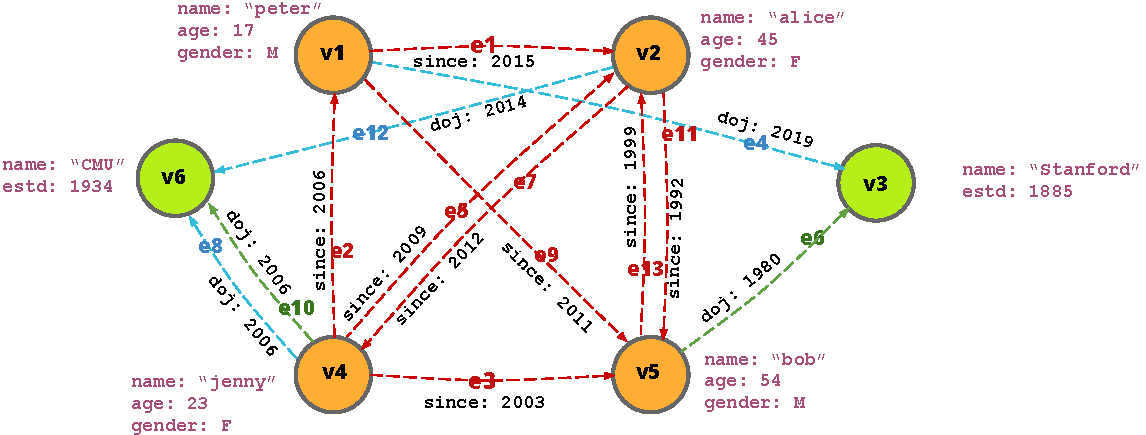
\includegraphics[scale=0.86]{img/property-graph}
	\vspace{-8pt}
	\caption{Running example graph.}
	\label{fig:runn}
	\vspace{-8pt}
\end{figure}

Figure~\ref{fig:runn} shows a graph data, that serves as our running example, in the property graph data model. A property graph consists of \emph{vertices} that represent entities and directed \emph{edges} between vertices that represent relationships between entities. Each vertex and edge has a particular \emph{label}, describing the high-level categories of vertices and edges. For example, in Figure~\ref{fig:runn}, vertices have labels: \texttt{PERSON} and \texttt{ORG}, while edges have labels: \texttt{FOLLOWS}, \texttt{WORKAT} and \texttt{STUDYAT}.

Similar to columns in relational tables, vertices and edges can have (key, value) \emph{properties}. Although the properties of vertices and edges do not need to adhere to a strict \emph{schema}, in practice many of these properties are often highly structured in the graph data, i.e., a similar set of properties will exist on all the vertices and edges of the same vertex and edge label respectively.

\section{Primary Storage Components in GDBMSs}
\label{sec:storage-components}

In every \gls{gdbms} we are aware of, the edges of a graph are stored in data structure called \emph{adjacency lists}~\cite{bonifati-adj-lists}. An adjacency list of a vertex $v$ is a list of \emph{adjacent} edges and \emph{neighbouring} vertices of $v$. In a \gls{gdbms}, each vertex has 2 adjacency lists - a \emph{forward adjacency list} containing all outward edges of that vertex, and a \emph{backward adjacency list} that holds all inward edges of the vertex. One can think of edges in the graph as a relational table, having 3 attributes, a source vertex, a destination vertex and an 8-byte edge ID. The adjacency lists can then be thought of as an \emph{index} on this relational table that is \emph{clustered} by either the source or destination vertex. In practice, often this index has a depth of 1 or 2, so given the ID of a vertex $v$, a system can access $v$'s list of edges in a small number of lookups. By having adjacency lists of a vertex in either direction, the system can access the list of outward and inward edges as well as the neighbouring vertices of $u$ in a constant-time lookup operation, which provides the core capability of fast joins on vertices to a \gls{gdbms}. 

Typically, a single-directional adjacency list of vertex $u$ is further clustered into sublists by the edge label of the edges. This enables extending a vertex through its edges with a \emph{particular} label in constant time. The rationale behind the sub-clustering is that many queries by applications have specific labels on query edges. Some systems further order the edge in the adjacency lists either by a property of adjacent edge or neighbour vertex or simply by neighbour vertex's ID. Sorting enables the system to access parts of lists in time logarithmic in the size of the adjacency list.

A \gls{gdbms} also stores properties that appear on the vertices and the edges. There are multiple solutions for storing properties. The most straightforward approach is to store properties in a \emph{key-value store} \cite{dgraph} and use the attribute key and the vertex or edge ID as the key into the store. Properties can also be stored in an interpreted attribute layout \cite{beckmann:sparse}, where a record of a vertex or an edge is a set of attribute-key pairs and is variable-sized. This is better suited than a fixed-size record owing to the randomness of properties over vertex or edge. Searching for a property in variable-sized records involves decoding and parsing the entire record until the matching attribute is found, which can be very slow. Yet another way of storing properties is in a doubly linked-list, as in Neo4j \cite{neo4j}, where the system keeps track of a pointer to the first property record of a vertex or edge and each subsequent property record points to the next. This is not a very optimized storage layout and does not localize and order the properties of vertices and edges. 

\section{Query Execution in GDBMSs}
\label{sec:operators}

In this section, we review the general execution of queries in a \gls{gdbms} by analyzing major operators used in the query plans. Though systems differ in their architectures and implementation of operators that they support for executing queries, there is similarity in their data access patterns. We use the Cypher query language \cite{cypher} to describe the queries we use in our examples. A user query typically consists of 3 parts, 1) a \texttt{MATCH} clause describes a subgraph query pattern $Q(V_Q, E_Q)$, where $V_Q$ and $E_Q$ are the query vertex and edge variables, that the system will match on the input graph; 2) \texttt{WHERE} clause contains a predicate $\rho$ over properties of the edges and vertices that the matched subgraph must satisfy; and 3) a \texttt{RETURN} statement that returns a projection of the variables in the match query or performs a group-by and aggregate information. The \texttt{MATCH}, \texttt{WHERE} and \texttt{RETURN} clauses of a cypher query effectively corresponds to the \texttt{FROM}, \texttt{WHERE} and \texttt{SELECT} clauses of SQL. Example \ref{ex:cypher-example} shows a typical query written in Cypher language, to query the example graph in figure~\ref{fig:runn}.

\begin{example}
	\vspace{5pt}
	\label{ex:cypher-example}
	Consider the following query. 
	{\em 
		\begin{lstlisting}[numbers=none,  showstringspaces=false,belowskip=0pt ]
		MATCH (a:PERSON)$-$[e:WORKAT]$\rightarrow$(b:ORG)
		WHERE a.age $>$ 22 AND b.estd < 2015
		RETURN *\end{lstlisting}
	}
	This query returns all the PERSON vertices and their workplaces, constrained to the condition that the \textsc{\char13}\texttt{age}\textsc{\char13} property of PERSON vertex has a value that is greater than 22 and \textsc{\char13}\texttt{established}\textsc{\char13} property of ORG vertex is less than 2015. a and b are query vertex variables while e is a query edge variable.
\end{example}
\vspace{-5pt}

The following are the major operators used for matching the subgraph pattern and evaluating predicates in a query.

\begin{itemize}
	
	\item \textbf{\texttt{SCAN}}: Scans a set of vertices and edges from the graph topology.
	
	\item \textbf{\texttt{NEIGHBOURHOOD JOIN}}: e.g. \texttt{EXTEND/INTERSECT} in Graphflow; \texttt{EXPAND} in Neo4j. On a high level, the neighbourhood join operator matches the subgraph query pattern $Q$, one edge at a time. Some systems, e.g Graphflow, can match cyclic queries by matching multiple edges at a time. The input to the operator is a partial match, $t$, that has matched $k$ of the query edges of $Q$. For each partially matched $t$, the operator extends $t$ by matching an unmatched query edge $e_q(u_q, v_q)$, where one of $v_q$ or $u_q$ has already been matched in $t$, say $v_q$ has already been matched. The \emph{join} happens by sequentially reading adjacent edges and neighbour vertices from (forward/backward) adjacency list of the matched $v_q$ one or more matched vertices of $t$, to produce a $k+1$-match. The output of the \texttt{JOIN} is the tuple $t$ with $e_q$ and $u_q$ filled.
	
	\item \textbf{\texttt{PROPERTY READER}}: (Vertex/Edge) property reader reads a property value of any vertex or edge that has been assigned to a variable in $V_Q$ or $E_Q$ of a partial match $t$, from the underlying property storage. 
	
	\item \textbf{\texttt{FILTER}}: Given the predicate $\rho$ from the \texttt{WHERE} clause and a partial match $t$ of $Q$, the \texttt{FILTER} operator omits $t$ from the result of the query if $t$ does not pass the predicate $\rho$.
	
\end{itemize}

\begin{figure}
	\hfill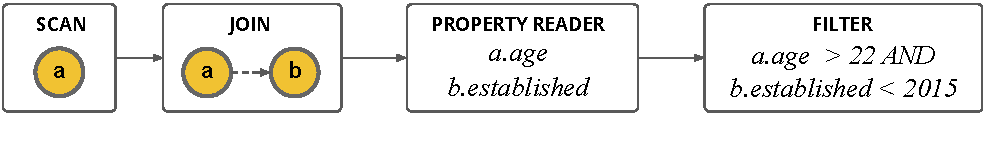
\includegraphics[scale=0.78]{img/ex-qp}\hfill
	\vspace{-10pt}
	\caption{Query plan for Example~\ref{ex:cypher-example}.}
	\vspace{-8pt}
	\label{fig:ex-qp}
\end{figure}

Figure~\ref{fig:ex-qp} shows one of the query plans that the system will generate to execute query in Example~\ref{ex:cypher-example}. It consists of the following sequence of operators: 1) \texttt{SCAN} operator that matches the variable $a$ in query to vertex in the graph having label \texttt{PERSON}; 2) \texttt{PROPERTY READER} reads the property \texttt{age} of the vertex matched to $a$; 3) \texttt{FILTER} operator filter out the partial match based on the contraint $a.age>22$; 4) \texttt{JOIN} operator matches $b$ by reading the forward adjacency list of $a$'s match; 5) \texttt{PROPERTY READER} reads the property \texttt{estd} of $b$'s match; and finally 4) another \texttt{FILTER} operator filters out the matched query pattern that do not confirm to the constraint $b.estd < 2015$.

\section{Guidelines and Desiderata}
\label{sec:guidelines}

We next outline a set of guidelines and desiderata for designing the physical data layout and query processor of a \gls{gdbms}.

\begin{guideline}[Edges are doubly-indexed.]
	\vspace{-5pt}
	Each edge appears in the forward adjacency list of that edge's source vertex and the backward adjacency list of its destination vertex. This results in a 2x replication factor in storing the topology of a graph in the system. This replication cannot be avoided by dropping an adjacency list in any one direction without hampering the capability to perform fast neighbour joins, which is one of the core feature of \gls{gdbms}s. So, we will also doubly index the edges in our design.
\end{guideline}


\begin{guideline}[Edge properties are read in the same order as edges in an adjacency list.]
	\label{ssec:edges-ordered}
	During the execution of a query, the \texttt{JOIN} operator will access the edges of a vertex $v$ in the order these edges appear in $v$'s (forward/backward) adjacency lists. If the query also needs to access the properties of these edges, the access to these edge properties will also be in the same order in which edges were read from the adjacency list. Given that the edges and edge properties are read in order, our first desideratum for the physical data layout and query processor is:
	
	\begin{desideratum}
		\label{des1}
		Store the properties of edges in the order in which edges are ordered in the adjacency lists and read the edges and their properties sequentially in the operators
	\end{desideratum}
	
\end{guideline}

\begin{guideline}[Vertices cannot be ordered to make access from all neighbour vertices sequential.]
	\label{gdln:vertices-unordered}
	Contrary to how the edges and edge properties can be strictly ordered for each of the adjacency lists, in general, there cannot be ordering on the vertices that completely localizes the access to neighbour vertices of every vertex and the properties of these neighbour vertices without prohibitive data replication. In general, if a vertex $v$ has $n$ neighbours, then $v$ and its properties need to be replicated $n$ times. Hence, localizing access to neighbour vertices and their properties should not be put in the desiderata of the system's physical data layout design. 	
\end{guideline}

\begin{guideline}[Access to vertex properties are random and many adjacency lists are very small.]
\label{gdln:fast-decompress}
Guideline~\ref{gdln:vertices-unordered} implies that the system should take it granted that access to the vertex properties will require random accesses and will not be sequential. For example, when joining a node $v$ with its neighbors and accessing the \texttt{age} property of each neighbor, the accesses will be to non-consecutive locations. Another property of real-world graphs is that adjacency lists of many vertices are very small because of the power-law distribution of adjacency lists. Systems should expect many very short adjacency lists, with only a few edges in them. Therefore during query processing with two or more joins, reading different adjacency lists and properties of these edges will require reading a short list followed by a random access and another short list, etc.

In an in-memory setting, which is the setting we focus on in this work, the focus with compression is not on achieving high compression ratios but to optimize for high decompression rates or to avoid decompression of data at all, as compressions schemes with slow decompression hurt performance. Our Guideline~\ref{gdln:fast-decompress} however also has further implications about the compression schemes that can be used in in-memory GDBMSs. Specifically, techniques that require decompressing blocks of data, say a few KBs, to only read a single property or a single short adjacency list can be prohibitively expensive.
%We designed our columnar data structures for in-memory \gls{gdbms}. For these data structures, the focus with compression is not on achieving high compression ratios but to optimize for high decompression rates or to avoid decompression of data at all.
\begin{desideratum}
\label{des:compression}
If compression is used, the system should be able to decompress arbitrary single elements in a compressed block in constant time.
\end{desideratum}  

\end{guideline}

\begin{guideline}[Graph data often has partial structure.]
	\label{gdln:graph-schema}
	Even though the property graph data model is semi-structured, in practice many graph databases stored in \gls{gdbms}s have a structure in different components, which \gls{gdbms}s can exploit. One reason this structure exists is that, as observed by prior works \cite{survey}, often the data in \gls{gdbms} comes from structured data in \gls{rdbms}. In fact, several of the \gls{gdbms}s from industry and some academics are actively working on defining a schema language for the property graph data model \cite{schema-validation-bonifati, defining-schema-hartig}. We identify three commonly appearing structure in property graph data:
	
	\begin{enumerate}
		
		\item \textbf{Edge label determines the source and destination vertex labels.} Often, edge labels in the graph data have a well-defined set of source and destination vertex label(s). This restricts the vertices to having inward or outward edges of only a definite set of labels. In our example graph, edges with label FOLLOWS only exists between vertices of label PERSON.
		
		\item \textbf{Edge label has fixed cardinality.} The number of edges of a particular label to which a source or destination vertex can be associated is a property of the edge label. We call this the \emph{cardinality} of an edge label. \emph{One-to-one} cardinality for a label $l_e$ means that each source vertex can be connected to at most one destination vertex through an edge with label $l_e$ and vice versa. \emph{Many-to-one} permits a single edge of a label from a source vertex but multiple edges to a destination vertex. Similar analogy can be applied to \emph{one-to-many} and \emph{many-to-many} cardinality edge labels.
		
		\item \textbf{Label determines properties on vertices and edges.} Similar to the attributes of a relational table, properties on an edge or vertex and the datatypes of these properties can \emph{often} be determined by its edge or vertex label. In our example graph, all vertices having label PERSON have 3 properties: name: \texttt{STRING}, age: \texttt{INT} and gender: \texttt{STRING}. As long as a significant fraction of vertices and edges with a particular label have a common set of properties, a system can exploit this structured to store these properties more efficiently. 
		
	\end{enumerate}
	
	Such structure in data provides an opportunity to design more efficient and simpler data structures for accessing the storage layer of \gls{gdbms}. Our second desideratum is:
	
	\begin{desideratum}
		Exploit the above three commonly appearing structure in the graph data to, 1) compress the data to save space, and 2) provide faster access to the data.
	\end{desideratum}
	
	\vspace{-10pt}
	However, not all data in graph databases have structure. As a working terminology, we will use the following terms:
	
	\begin{itemize}
		\item \textbf{Structured/unstructured edge:} An edge of a particular label, that follows above-mentioned points \ref{gdln:graph-schema-rule1} and \ref{gdln:graph-schema-rule2}, is called an structured edge. An edge that is not structured, is called an unstructured edge.
		
		\item \textbf{Structured/unstructured property:} A structured property is a property on a vertex or edge that, 1) can be determined by the vertex type or edge label of that entity; 2) appears in a significant fraction of the vertices of edges of a particular label; and 3) have the same data type in all its occurrence. Any property that is not a structured property, is considered unstructured.
		
	\end{itemize}
	
	
	We focus on optimizing the storage of structured part of the graph data in this thesis. It forms an interesting research topic to optimize a system for unstructured part of graph data. A standard approach is to serialize the key, datatype and value of each property in variable-length records. Structured property storage can, however, be optimized to benefit memory footprint as well as access performance.
	
\end{guideline}

\begin{guideline}[Queries read a small subset of the vertex or edge properties]
	In order to understand the nature of queries user ask on \gls{gdbms}, we conducted a survey of 100 StackOverflow questions containing openCypher queries. We focused on queries of analytical nature and discarded transactional ones like insert, delete and update. We observe the following: 
	
	
	\begin{itemize}
		
		\item Out of the 100 queries, 68 accessed at least one of the properties on a vertex or an edge. Of these, 61 accessed vertex properties and 13 accessed edge properties.
		
		\item Only 11 queries returned all the properties of a query edge or vertex, while 35 of them return specific properties.
		
		\item Average number of properties accessed by those queries that explicitly return a set of properties was only 1.6.
		
	\end{itemize}
	
	We can observe that vertex properties are more popularly accessed as compared to edge properties and most of the queries only access 1 or at most 2 properties. This observation leads to our third desideratum:
	
	\begin{desideratum}
		Allow fast access to individual properties of multiple vertices instead of all properties of a single vertex.
	\end{desideratum}
	
\end{guideline}


\chapter{Columnar Storage}
\label{c:columnar-storage}

In this chapter, we explore the application of columnar data structures for different storage components of  \gls{gdbms}s to meet the desiderata we outlined in Chapter~\ref{c:guidelines}. Section \ref{sec:vertex-property-columns} describes the design of columns to store vertex properties and a new compact vertex ID scheme that accompanies the design. In Section \ref{sec:edge-property-columns}, we start by describing two columnar storage designs to store edge properties and their pros and cons. Then, we propose a third design, Single-directional property pages, that is a sweet spot between the earlier two designs and the one we adopt for storing edge properties. Similar to Section~\ref{sec:vertex-property-columns}, we describe a novel and compact edge ID scheme that accompanies our design from edge property columns. In Section~\ref{sec:single-cardinality-cols}, we describe a storage optimization that involves storing edges with cardinalities 1-1, 1-n, n-1 in vertex property columns instead of using the more heavy-weight CSR columnar structure. We address how to compress the data stored in these columnar structures in Chapter~\ref{columnar-compression}.
%Section~\ref{sec:storage-optimizations} describes several storage optimizations to the adjacency lists to reduce the system's memory footprint without sacrificing query performance, using different type of structure that may exist in input graphs that we observed in Guideline~\ref{gdln:graph-schema}.

\section{Columnar Storage for Vertex Properties}
\label{sec:vertex-property-columns}

\begin{figure}
	\hfill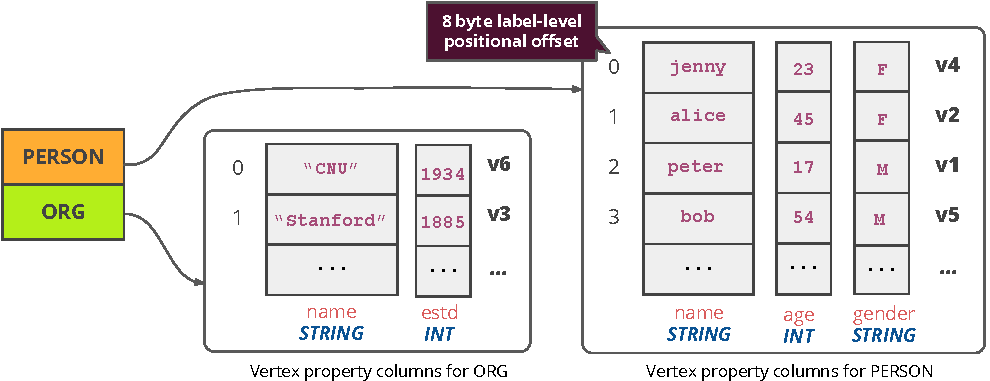
\includegraphics[scale=0.85]{img/vpcols}\hspace*{\fill}
	\caption{Vertex property columns for the graph in Figure~\ref{fig:runn}.}
	\label{fig:vpcols}
\end{figure}

Columnar data-structures can be directly used for storing vertex properties. Let $(lv_1, lv_2, ...)$ be the vertex labels in a graph. Let $p_{i,1},  p_{i,2}, ... p_{i, n}$ be the structured vertex properties of $lv_i$, each with a specific datatype $d_{i,j}$. We define a \emph{vertex property column} for each $p_{i,j}$, having a fixed data type $d_{i,j}$. Each column stores the value of a single property $p_{i,j}$ for all vertices having $lv_i$ at consecutive locations. All property values of a particular vertex $v$ with label $lv_i$ is located at the same positional offset for each column for $p_{i,j}$. 

% reading a property.

Ideally, the property value of a vertex should directly be read using the ID of the vertex as the positional offset in the column. However, \gls{gdbms} typically gives globally unique 8-byte consecutive IDs to all the vertices in the system, irrespective of their labels. That means ID 0 can be given to a vertex with label PERSON and 1 to a vertex with label ORG and 2 to another vertex PERSON etc. We cannot use this ID scheme as the positional offset for the above design. One possible solution is to maintain a map for each label, from each vertex $v$'s \enquote{global} ID to a \enquote{local} label-level positional offset, which is unique only among all vertices with the same label as $v$. This requires extra storage for maintaining the map and one level of indirection when accessing the vertex properties. Instead, we adopted an ID scheme where each vertex is identified by a \emph{\textbf{(vertex label, label-level positional offset)}} tuple in the system in place of global vertex ID. This allows direct access to the properties by using the local positional offset which now is part of the vertex ID. However, using this new vertex ID scheme requires materializing 2 pieces of information in the adjacency lists - a vertex label and a local positional offset, compared with a single global vertex ID. This may increase the memory overhead  if the local positional offsets and the global vertex ID are of the same size. However, we will show in Section \ref{sec:storage-optimizations} that we can often avoid storing the vertex labels with vertex IDs and even save space by using fewer bytes for local positional offsets than the bytes needed by the global vertex IDs.

For reference, Figure~\ref{fig:vpcols} shows a set of vertex property columns for our example graph in Figure~\ref{fig:runn}. It has 2 set of columns one for each vertex label, with a column for each structured property of the label. The global vertex IDs on the right of the set of columns of a vertex label indicates the positional offset at which the properties of a particular vertex are located in the columns of a family. For instance, the properties of vertex $v2$ appear at offset $1$ in columns of PERSON's family. By the new vertex ID scheme, $v2$ is identified as \texttt{PRESON:1}. 


% updates.

Recall from Guideline~\ref{gdln:vertices-unordered} that in general, reading the properties of vertices (specifically when reading the properties of neighbors of a vertex) cannot be localized without prohibitive replication. In light of this guideline, we adopt a simple and efficient additions and deletion scheme for of vertex properties and vertices. Deleting  the property of vertex $v$ is handled by setting the property at $v$'s positional offset to NULL.  Deleting $v$ is handled by setting all of $v$'s properties to NULL and adding $v$'s positional offset to a list of ``recycled'' offsets. When a new vertex $v$ is added, the system generates an ID by using a recycled offset if one exists or gives a new consecutive positional offset (i.e., increments the maximum positional offset by 1). Updating $v$'s property is handled by overwriting the value in the property column for $v$'s positional offset. All of these operations are very efficient involving only random access to different locations in columns.

\section{Columnar Storage for Edge Properties}
\label{sec:edge-property-columns}

Recall from Guideline~\ref{ssec:edges-ordered} that edges and edge properties  are read by the \texttt{JOIN} operators in the order they appear in the adjacency lists. \gls{gdbms}s store the edges, i.e the (edge ID, neighbour vertex ID) pairs, consecutively in adjacency lists, through double indexing. Ideally, edge properties should also be stored in the same order. In this section, we begin by presenting two columnar storage designs for storing edge properties which can be seen as opposite ends of a design spectrum. The first design, {\em edge property columns}, is optimized for \emph{storage} and does not replicate the edge properties. The second design, {\em double-indexed property lists}, is optimized for \emph{performance} through double indexing of the edge properties. We then describe a third design, {\em single-directional property lists}, that can be seen as a sweet spot between the previous two designs, which localizes the reads in one direction without any replication. However, this natural third design has several limitations, which we address in our fourth design, {\em single-directional property pages}, which is adopted in Graphflow. 

% However, this also requires double indexing, which is expensive as each property needs to be replicated. 
\begin{figure}
	\vspace{-20pt}
	\hspace*{-20pt}
	\begin{subfigure}{0.45\textwidth}
		\vspace{14pt}
		\centering
		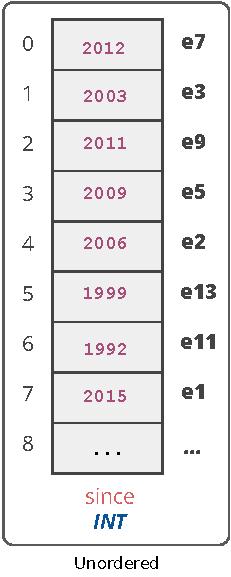
\includegraphics[scale=0.69]{img/sol1}
		\captionsetup{justification=centering}
		\vspace{12pt}
		\caption{Edge Property Columns}
		\label{fig:sol1}
	\end{subfigure}
	\begin{subfigure}{0.55\textwidth}
		\centering
		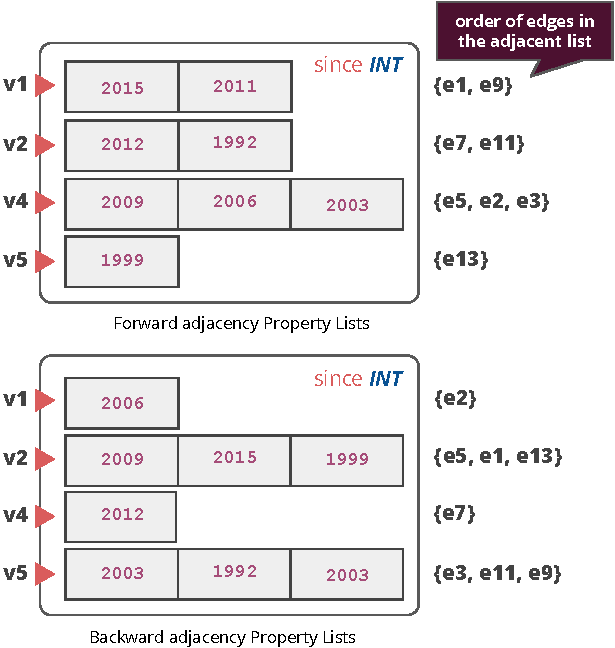
\includegraphics[scale=0.69]{img/sol2}
		\captionsetup{justification=centering}
		\caption{Double-indexed Property Lists}
		\label{fig:sol2}
	\end{subfigure}
	\captionsetup{justification=centering}
	\caption{Storing edge properties of FOLLOWS edges in the Edge Property Columns and Double-indexed Property Lists.}
	\label{fig:sol1and2}
\end{figure}


\subsection{Edge Property Columns and Double-Indexed Property Lists}

\noindent {\bf Edge Property Columns (Nonsequential reads, no replication):} One possibility is to use the columnar storage design similar to that for storing the vertex properties. That is, we have one edge property column for each $q_{i,j}$, where $q_{i,j}$ is a structured property of edge label $le_i$. Edges in the system with this solution can be identified as \emph{(edge label, label-level positional offset)}. However, such a design would not localize the properties of the edge according to their appearance in the adjacency lists, so cannot provide sequential reads when reading the edge properties. Figure~\ref{fig:sol1} shows how this particular design would look like. The figure shows a column storing property \texttt{since} of FOLLOWS edges. The property values are not ordered. For our example, the forward adjacency list of \texttt{v4} contains edges \texttt{e5}, \texttt{e2} and \texttt{e3}, whose \texttt{since} property values (at positional offsets 3, 4 and 1) are not stored consecutively in the edge property column. 

\noindent {\bf Double-Indexed Property Lists (Sequential reads in both directions, 2x replication):} An alternative solution is to directly mimic the storage of the adjacency lists for storing the edge properties. For each vertex $v$ that has edges with a label $l_i$, and each $q_{i,j}$, we store the edge properties in the \emph{forward property lists} and \emph{backward property lists}. This provides sequential read of properties. For example, a query that is reading the forward (backward) adjacency list of $v$ can read the edge property values of the edges sequentially from the forward (backward) adjacency property list of $v$. Figure~\ref{fig:sol2} shows the forward and backward property lists for edgel label \texttt{FOLLOWS} in our example graph in Figure~\ref{fig:runn}. However, this design requires replicating each edge property twice. In addition, if the original adjacency lists are sorted, then all the property lists need to be sorted too in the same way, which would make updates slower. 

\subsection{Single-directional Property Pages}

\begin{figure}
	\hfill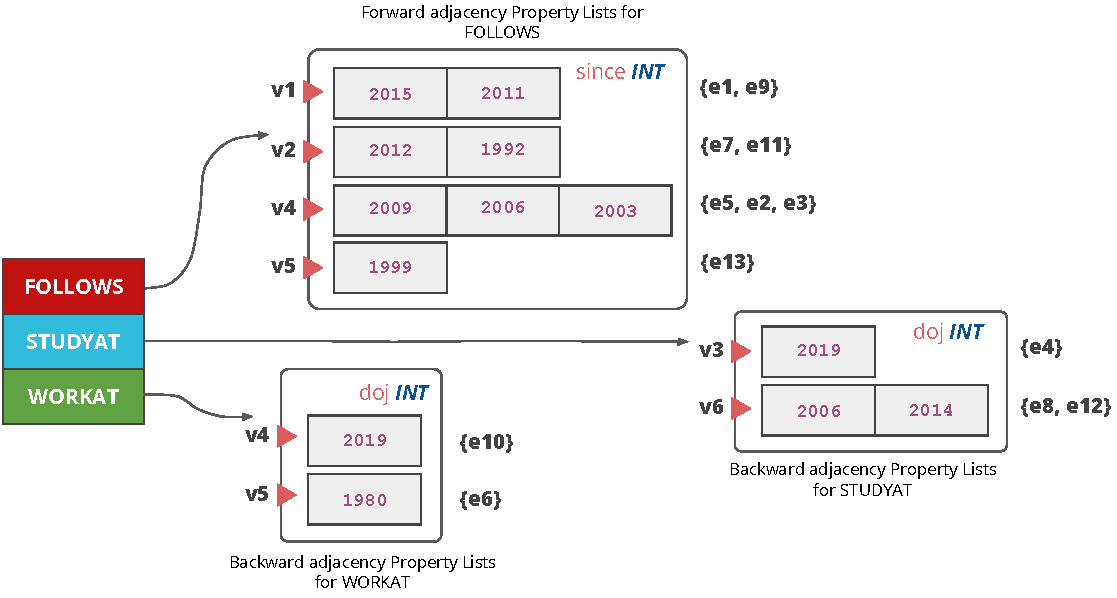
\includegraphics[scale=0.78]{img/single-dir-prop-list}\hspace*{\fill}
	\captionsetup{justification=centering}
	\caption{Single-directional Adjacency Property Lists}
	\label{fig:single-dir-prop-list}
\end{figure}

A natural middle ground between edge property columns and double-indexed property lists is to store only one of the forward or the backward property lists. We call this design \emph{single-directional adjacency property lists}. Suppose the system indexes the properties of the edges with label $l_i$ in the forward direction. Then, the edge properties can be read sequentially in the forward direction. However when reading the edges of a vertex $v$ in the backward direction, then the edge properties will not be sequential. Figure~\ref{fig:single-dir-prop-list} shows the Single-directional Adjacency Property Lists for storing the properties of the example graph in Figure~\ref{fig:runn}. In the example, edge properties in the family of FOLLOW and WORKAT labels are stored in the forward adjacency property lists, while in STUDYAT the properties are in the backward adjacency property lists. In this design, reading the edges in the backward direction requires that given the ID of an edge $e$, the system is able to locate the positional offset of $e$ in the forward direction. This requires a new edge ID scheme. Specifically, the conventional globally consecutive edge IDs cannot be used to access the properties quickly as they do not contain information about positional offsets. We next describe a new edge ID scheme to achieve this. Then we talk about some important limitations of single-directional property lists, which we address in a new design.

To access a property of an edge $e$ having label $le_i$, we need 3 pieces of information; 1) $q_{i,j}$; 2) source vertex if the $q_{i,j}$'s values are stored in the forward adjacency property lists, else destination vertex; and 3) the list-level positional offset of $e$ in that property list. For instance, in figure~\ref{fig:single-dir-prop-list}, \texttt{since} property of $e2$ can be accessed knowing $v4$ (source vertex of $e2$) and offset of $e2$ in $v4$'s forward adjacency property list, i.e 1. We adopt a new edge identification scheme that identifies the edge in the system by a tuple having 4 components: \textbf{\emph{(edge label, source vertex, destination vertex, list-level positional offset)}}. In our new scheme, the $e2$'s ID will be given as \texttt{FOLLOWS:v4:v1:2}, where $v4$ and $v1$ are the source and destination edges of $e2$. These edge IDs provides us with compact storage too. Most of the components need not be stored in the adjacency lists and the edge ID can be constructed during query execution by reading as few as only the neighbour vertex's local positional offset in the property list. 

\noindent {\bf Limitation of single-directional property lists:} Though single-directional adjacency property lists are a good middle-ground solution, it has an important limitation. Suppose that the property list for property $q_{i,j}$ of edge label $le_i$ is indexed in the forward direction. If the original adjacency lists are sorted,  any insertion or deletion can change a large number of, possibly all of the positional offsets of every edge in the adjacency list. Suppose an edge is inserted to the beginning of $v$'s forward adjacency list $L_f$. This requires first calculating a map of old and new positional offsets of the edges in $L_f$, then searching through each backward neighbor of $v$ and finding each edge in the backward adjacency list and updating its positional offset. A similar problem exists when an edge is deleted. If the original edges are not sorted, then insertions can be handled easily but handling deletions is challenging. The system has two options for deletions. First, the system can directly delete the edge $e$, which again can change the positional offsets of as many as $|L_f|$ edges. Instead, the system can thumbnail $e$'s positional offset and recycled $e$'s positional offset as was described for vertex deletions. However, this is also expensive. In contrast to keeping a single list of recycled IDs as in vertex property columns, the system now needs to keep track of recycled positional offsets for each vertex, so up to $|V|$ many recycled IDs list.

\begin{figure}
	\hfill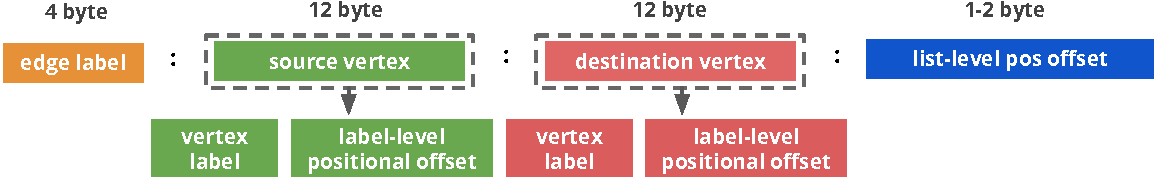
\includegraphics[scale=0.78]{img/edge-scheme}\hspace*{\fill}
	\captionsetup{justification=centering}
	\caption{Components of the new edge identification scheme.}
	\label{fig:edge-scheme}
\end{figure}

\noindent {\bf Single-directional property pages:} To address the above limitation, we take $k$ property lists (by default 64) and store their properties in a property page. Properties in a property page is not necessarily stored consecutively. However, because we use a small value of $k$ and adjacency lists of many vertices are short in many real world datasets, these properties are stored in close-by memory locations. We do not sort these pages when the original adjacency lists are sorted and keep a recycled ID list for each page, avoiding the cost of sorting and the maintenance of list-level recycled ID lists. We can use the same edge ID scheme we described above, except the positional offsets now identify the properties of edges in property pages, instead of property lists. Suppose again that the property $q_{i, j}$ is stored in the forward direction (though properties of $k$ lists are grouped). Given an edge $e$ in the scheme from Figure~\ref{fig:edge-scheme}, we can take the source vertex's label-level positional offset and divide it by $k$ to identify the page in which $e$'s $q_{i, j}$ property is. Within this page, the property can be accessed with a single lookup using the positional offset of $e$.

\begin{figure}
	\hfill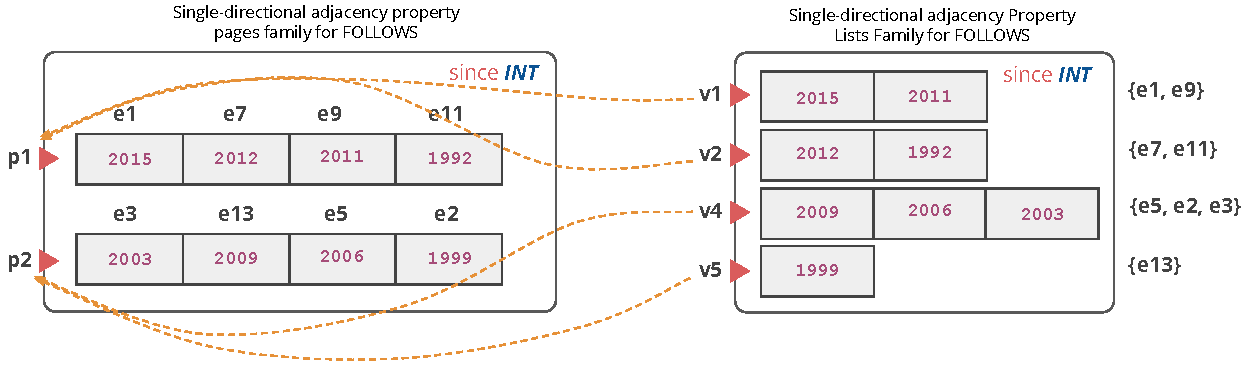
\includegraphics[scale=0.78]{img/paged}\hspace*{\fill}
	\captionsetup{justification=centering}
	\caption{Mapping single-directional adjacency property lists to single-directional adjacency property pages for since property in Figure~\ref{fig:runn}.$n=2$.}
	\label{fig:paged}
\end{figure}

%The mapping from a property list to its corresponding page is straightforward. Single-directional adjacency property list for vertex $v$ and property $q_{i,j}$ maps to the $i$th page for property $q_{i,j}$, where $i$ is mod $n$ of $v$'s local positional offset. The benefit of using pages comes from it being unordered. This makes new edge insertions easy as now, the new edge properties get appended into their respective pages or recycle the location of an already deleted edge, similar to how insertions happen in vertex property columns. 

Figure~\ref{fig:paged} shows the mapping of a single-directional adjacency property lists to single-directional  property pages for $n=2$. The paged edge property column has two pages that stores the property values from vertex groups $(v1,v2)$ and $(v3,v4)$ respectively, assuming that the local positional offset of $vi$ is $i$ and $pi$ is the $i$th property page for \texttt{since} property. 
%The value of $n$ is chosen such that edges' property values are not too far apart from each as they were stored in %the property lists. This reduces the cache miss to occur with \emph{each} access of a value in a page. Hence, the value of $n$ is dependant on 3 factors: 1) the cache line size; 2) width of an element in the page, and 3) the average number of edges in the adjacency lists. Ideally, the value of n is optimum in the range $[32, 512]$. 
We show in evaluation that single-directional  property pages is similar, about 1.2x slower, in performance to single-directional property lists in read-heavy stress tests and about 4.5x faster than using edge property columns. 

\section{Vertex Property Columns for Single Cardinality Edges}
\label{sec:single-cardinality-cols}

When an edge label has 1-1, 1-n, n-1  cardinality then vertices can have at most one edge in at least one direction. We refer to these edges as {\em single cardinality edges}. For instance, in our Figure~\ref{fig:runn} example graph, edge label STUDYAT and WORKAT have the cardinality \texttt{n-1}, i.e., a PERSON vertex can have at most one STUDYAT's and WORKAT's edge (in the forward direction). Therefore, instead of storing the single edge in these adjacency lists in the last level of the 2-level CSR structure, we can store them as a \emph{property} of either the source of destination vertex and directly access them using the positional offsets of the source or destination vertex of the edge. This both saves space, as we do not need to store the CSR offsets, and we can directly access these properties with 1 instead of 2 random lookups in a CSR. Figure~\ref{fig:single-cardinality-cols} shows the edges of edge label STUDYAT and WORKAT, from our example graph, and their properties being stored as the special property of vertex type PERSON.

%Benefits of storing edges as special vertex properties is two-fold, Figure~\ref{fig:single-cardinality-cols} shows the STUDY AT edges stored as the special properties of PERSON vertices. Moreover, the properties of such an edge $e$ can also be stored in structures similar to the vertex property columns, instead of single-directiional property pages. These properties are hence, accessed by vertex $v$'s local positional offset, instead of page-level positional offset, where $v$ is the vertex whose special property the edge is. Thus, we do not need page-level positional offsets for the edges of single cardinality edge labels.

\begin{figure}
	\hfill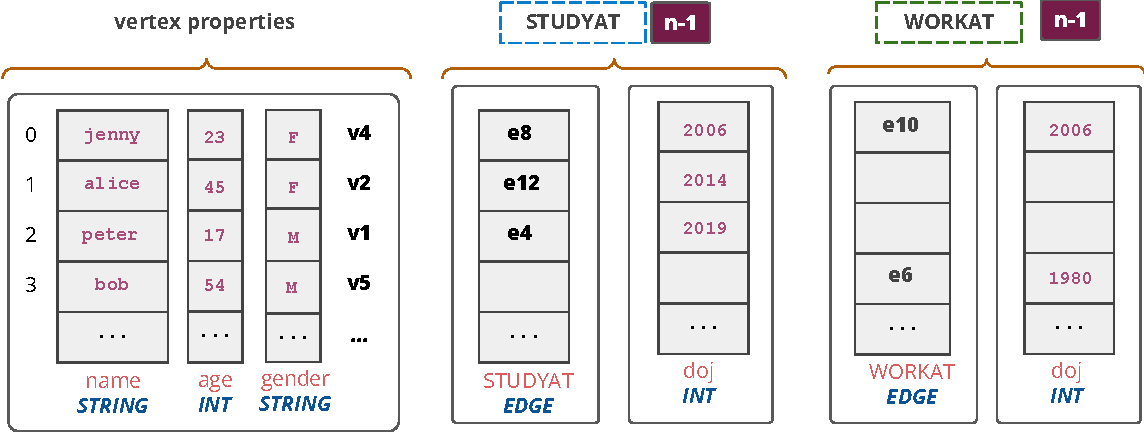
\includegraphics[scale=0.78]{img/single-cardinality-cols}\hspace*{\fill}
	\captionsetup{justification=centering}
	\caption{Storage of edges having single cardinality edge label STUDYAT and WORKAT as special property of PERSON.}
	\label{fig:single-cardinality-cols}
\end{figure} 




\chapter{Columnar Compression}
\label{columnar-compression}

Compressing data stored in columns and query processing directly on compressed data have been extensively studied in the context of column-oriented \gls{rdbms}s. 
These techniques are directly relevant to our work. However, not all columnar compression techniques can be directly applied to the data-structures that we introduced in Chapter~\ref{c:columnar-storage}. Recall our Desideratum~\ref{des:compression} that in the context of in-memory GDBMSs, we are interested in compression schemes that either avoid decompression at all or decompress arbitrary single elements in a compressed block in constant time. For example, schemes such as run-length encoding are not suitable for in-memory GDBMSs because it is not possible to decompose the value of an arbitrary element in constant time. We begin in Section~\ref{sec:col-existing} by reviewing a number of existing compression techniques that satisfy this constraint and where they can be applied in GDBMSs. In Section~\ref{sec:storage-optimizations} we discuss opportunities where we can compress our adjacency lists, i.e., the storage of (edge ID, neighbour ID) pairs, given our new ID schemes. Finally, in Section~\ref{sec:null}, we discuss the shortcomings of directly applying existing null compression schemes from columnar RDBMSs to compress null values or empty lists in GDBMSs and propose a new \emph{prefixSum-based null compression} scheme that is suitable for GDBMSs.

\section{Directly Applicable Compression Techniques}
\label{sec:col-existing}

%We designed our columnar data structures for in-memory \gls{gdbms}. For these data structures, the focus with compression is not on achieving high compression ratios but to optimize for high decompression rates or to avoid decompression of data at all. There has been much research that studies compression techniques from the point of avoiding eager decompression of compressed data \cite{westmann-comp, dat-comp}. \cite{abadi-col-comp} abstracts out the high-level properties of a compression algorithm and use this information in query executor to operate directly on compressed data whenever possible. Our's is an identical requirement in the sense that operating directly on compressed data can avoid CPU overhead and increases the read throughput while reading from adjacency lists and property stores.
%
%The design of vertex and edge property columns as described in sections \ref{sec:vertex-property-columns} and \ref{sec:edge-property-columns}, allows for random access of property values based on the positional offset in a column. Random lookups in a column can be performed intuitively once we decompress the entire column or a part of it. However, this involves the additional cost of decompressing elements that are not required to be read, thereby wasting CPU cycles. We can avoid this cost by randomly acessing elements from the compressed column, which is a step ahead of operating directly on the compressed data. 
Random access to a compressed column is possible only if the elements of a column are encoded in \emph{fixed-length codes}, i.e. using a fixed number of bits, instead of variable-length codes. Several existing schemes, such as dictionary encoding, leading 0 suppression, bit vectors, and frame of reference produces fixed length codes. We review dictionary encoding and leading 0 suppression below, which we have integrated in our implementation. We refer the readers to references~\cite{abadi-col-comp, goldstein:for, lemire:integer} for details of other schemes.
We next review several of existing techniques that produce fixed length codes.

%The only columnar compression techniques that keep the data in fixed-width bits are \emph{dictionary encoding} and \emph{bit-vector encoding}. Whereas, related techniques, \emph{Prefix Supression} and \emph{Frame of Reference (FOR)}, can be adopted to encode elements in fixed-bitwidth to make them appropriate for our case. For each of these techniques, we give a brief description of the technique and state its characteristics that makes it suitable for our use-case. We also give a high-level implementation of how a technique is used in our system.
\noindent \textbf{Dictionary encoding:} The dictionary encoding is perhaps the most common encoding scheme to be used in \gls{rdbms}s~\cite{abadi-col-comp, boncz-comp}. At a high-level, this scheme maps a domain of values into more compact and shorter representations using a variety of schemes \cite{boncz-comp, dat-comp, abadi-col-comp}. Some of these schemes produce variable-length codes, such as Huffmann encoding, and others use fixed-length codes, such as the one described in reference\cite{abadi-col-comp}. These techniques are often used to encode \texttt{STRING}s into 64-bit integer values or any categorial property into a small number of fixed-length bits. Different schemes can further pack these bits into bytes. In our implementation, we use dictionary encoding to map any categorial property $p$ that takes on $z$ different many values to  $\lceil log_2(z)/8 \rceil$ bytes (so we pad $log_2(z)$ bits with 0s to have a fixed number of bytes).
	
%\noindent \textbf{Bit-vector encoding:} The bit-vector encoding scheme is used to encode columns with small number of unique elements. It encodes the column by having $n$ bit-strings, one for each unique element. A bit-string associated to the value has the bit set at positions where that value appears in the column. Accessing a random location $i$ in a column compressed by bit-vector involves inspecting the $i$th position of each bit-string till a set bit is found. Inspecting \emph{all} the bit-strings adds to the overhead which increases with the number of unique values in the column. Hence, encode a column using bit vectors only when the unique values are less than 50.
	
\noindent  \textbf{Leading 0 Suppression:} Given a block of data, this scheme omits storing leading zero bits or in each value in the block \cite{beckmann:sparse}. Each value is, hence, encoded in a variable number of bits along with the count of bits used for storing the value. For an integer value 12, the number of bits in which it can be stored is 4, instead of default 32. There are both variable-length and fixed-length variants of this scheme. We adopt a fixed length version where for storing labels and positional offsets in both edge and vertex IDs (though it is trivial to apply to vertex and edge properties as well). Specifically, if there $max_v$ many vertices of a particular label, we store the positional offsets in $\lceil log_2(max_v)/8\rceil$ many bytes instead of 8 bytes. Similarly, if the maximum size of a property page of an edge label is $k$, for all for all the associated edges, we use $\lceil log_2(k)/8\rceil$ many bytes for the page-level positional offset of the edge ID. Often the forward adjacency lists of many edge labels are quite small (even the maximum length one), and we store the positional offsets with a few bytes, instead of 4 bytes. Similarly if there are $max_{\ell}$ many different labels, we store labels as in $\lceil log_2(max_{\ell})/8\rceil$ many bytes. That said, during query processing and accessing properties, the  labels, positional offsets of vertices, and positional offset of edges are stored as 4, 8 and 4 bytes, respectively.

%\begin{enumerate}
%		\item To make this encoding byte-aligned and easy to decompress, we store the values in variable bytes instead of in variable number of bits. Hence, an integer value can be encoded with either 1, 2, 3 or 4 bytes, with two extra bits needed to store the number of bytes. 
%		\item We do not encode each element of the column separately in variable-bitwidth. Instead, the element is encoded in the number of bytes that is sufficient to encode the largest element in a column or a block in column. The number of bytes for encoding an element is, hence, given by $\lceil log_2(max_v+1)/8\rceil$, where $max_v$ is the maximum element in the column or block. The resultant column now has fixed-bitwidth elements and does not need to store an extra 2 bits for the number of bytes used.
%	\end{enumerate}

%\noindent  \textbf{Frame Of Reference(FOR): }This technique is similar to the previous, instead each element $e$ is stored as NULL supressed $e-b$, $b$ is called the \emph{base value} of the column or block. Generally, for an integer column, its smallest element is take as the base value. FOR is effective when the elements of column are clustered.
	
\section{Compressed Storage of Edge and Vertex ID Pairs in Adjacency Lists}
\label{sec:storage-optimizations}

We next discuss how to compress the edge ID and vertex ID pairs in the adjacency lists. Our new ID schemes from Sections \ref{sec:vertex-property-columns} and \ref{sec:edge-property-columns} decompose the IDs into multiple small components, which enables us to factor out most of these components, when the data depicts some structure. 

Recall that the ID of an edge $e$ in our new edge ID scheme contains 4 components: (i) edge label; (ii) source vertex ID; (iii) destination vertex ID; and (iv) positional offset of the properties of $e$ in property pages. Recall also that then ID of a vertex $v$ contains 2 components: (i) vertex label; and (ii) (label-level) positional offset. First, both the source and the destination vertex IDs inside the edge ID of (edge ID, neighbor ID) pairs can be omitted. This is because the source (destination) vertex ID is implied by the offset of the pair in the forward (backward) adjacency list and the destination (source) vertex ID is the neighbor ID, which is already stored in the pair. Second, we do not have to store the labels of the edges as in our storage of the adjacency lists because recall that we store a different CSR-like structure for each edge label. Therefore the only parts that need to be stored are positional offsets for edge IDs, and vertex label and positional offsets of neighbor IDs. We next discuss further cases when the structure and multiplicities of edges allows us to factor some of these components out: 
%Finally, the positional offset can be stored cheaply as often they are not more than 1 or 2 bytes hence. This follows from the fact that the number of edges in most of the adjacency list is relatively small (by the power-law) and so are the number of elements in each page. 

%To sum up, each entry in the adjacency list stores a small (1-2 byte) positional offset and the neighbour vertex ID which itself comprises of vertex label and local positional offset. We now present some common scenarios that allow for even further compaction by choosing to omit to store certain components:

\begin{figure}
	\centering
	\begin{tikzpicture}[node distance=3cm]
	\node (edge) [io] {edge $e$};
	\node (dec1) [decision, below of=edge] {has 1 neighbour label?};
	\node (p1) [process, below of=dec1] {Do not store neighbour vertex label};
	\node (p2) [process, right of=dec1, xshift=1cm, yshift=-2.8cm] {store neighbour vertex label};
	\draw [arrow] (edge) -- (dec1);
	\draw [arrow] (dec1) -- node[anchor=east] {yes} (p1);
	\draw [arrow] (dec1) -| node[anchor=south] {no} (p2);
	\end{tikzpicture}
	\captionsetup{justification=centering}
	\caption{Decision tree to store neighbour vertex's label in the Adjacency lists.}
	\label{fig:dec1}
\end{figure}

\begin{itemize}
	\item \textbf{Edge label determines a single neighbour vertex label.} In this very frequent case, an edge label is between pairs of nodes when the sources or destinations (or both) can have a single label. For instance, in our example graph, \texttt{FOLLOWS} edges are between vertices having the label \texttt{PERSON}. In this case, we can factor out the vertex label component of neighbor ID.
		
	\item \textbf{Edges do not have properties:} This is also a frequently appearing case. That is the edges with a particular label do not have any structured or unstructured properties. In this case, notice that the edges do not need to be identifiable at all as the system will never access properties of these edges. Therefore, what distinguishes two edges are their neighbor IDs and edges with the same IDs are simply replicas of each other and are stored twice. Therefore, we can omit storing the positional offsets of edge IDs.
	
	\item \textbf{Single cardinality edges:} Recall from Section~\ref{sec:single-cardinality-cols} that the properties for single cardinality edges can be stored in vertex property columns. So by using the source or destination vertex IDs, we can directly read properties. Therefore, we can omit storing any positional offsets. 
		
\end{itemize}

\begin{figure}
	\centering
	\begin{tikzpicture}[node distance=3cm]
	\node (edge) [io] {edge $e$};
	\node (dec1) [decision, below of=edge] {single cardinality?};
	\node (p1) [process, below of=dec1] {Do not store positional offsets};
	\node (dec2) [decision, right of=dec1, xshift=1.2cm] {has properties?};
	\node (p2) [process, right of=dec2, xshift=-0.5cm, yshift=-3cm] {store positional offsets};
	\draw [arrow] (edge) -- (dec1);
	\draw [arrow] (dec1) -- node[anchor=east] {yes} (p1);
	\draw [arrow] (dec1) -- node[anchor=south] {no} (dec2);
	\draw [arrow] (dec2) |- node[anchor=south, xshift=-1cm] {no} (p1);
	\draw [arrow] (dec2) -| node[anchor=south] {yes} (p2);
	\end{tikzpicture}
	\captionsetup{justification=centering}
	\caption{Decision tree to store edge's positional offset in the Adjacency lists.}
	\label{fig:dec2}
\end{figure}

All of the above cases arise frequently in real world graph data. For example, in the \gls{ldbc} dataset~\ref{fig:ldbc-schema}, 10  out of 15 many edge labels determine a single source and destination neighbour label, 10 many do not have any properties, 8 many have single cardinality edges. In all, 10 many of them are not required to store any neighbour vertex's labels and positional offset. This implies that we only store neighbour vertex's positional offset for such edges in the adjacency lists, which can be stored with as few as 4 bytes.

Figures~\ref{fig:dec1} and ~\ref{fig:dec2} summarizes these cases in a decision tree that instruct when to omit storing certain components.

% **** Let's not call NULL compression but "trailing 0 omission" and I think let's not talk about factoring things out 
%Using the new identification scheme and further applying the above-mentioned optimizations, the adjacent edges and neighbour vertices in adjacency lists by as less as a single piece of information. We can still further reduce the memory footprint of adjacency lists by applying compression on components of the edge that has to be stored after removing unnecessary ones. We use \emph{fixed-bitwidth NULL compression}, which we describe in Section~\ref{sec:col-existing}, to compress the components of edge in the adjacency lists. Using this technique, a particular component of each edge in an adjacency list is encoded as fixed-width elements by removing a common number of leading zero bytes (that will be determimined by the maximum element) from each of them. For example, if an adjacency list has edge $[e1, e2, e3, e4, e5]$ with the neighbour vertex labels $[1, 2, 1, 1, 2]$, then the neighbour vertex label is encoded in 1 byte in the adjacency list, instead of usual 4-byte INT. Similarly, if the same set of edges have neighbour's local positional offsets $[1000, 2000, 3000, 2, 1]$, then each offset is stored in 2 bytes in the adjacency list.

%We show the decrease in memory footprint of the adjacency lists, with each optimization, over the LDB SnB dataset, with more than 1 billion edges, in Chapter~\ref{c:evaluation}. Our evaluations reveal that the new scheme with opportunities to perform immense compaction and compression can reduce the size of adjacency lists by upto 94x, storing barely over 6 bytes of data per indexed edge in the system.

\section{NULL Compression}
\label{sec:null}

Edge and vertex properties can often be quite sparse in real-world graph structured data. Similarly in many adjacency lists, due to the power-law nature of the degree distributions, a significant fraction of vertices can have empty forward or backward adjacency lists. Both the property sparsity and empty lists can be seen as different columnar structures containing null values, which can be compressed.

%Owing to the nature of property graph data, one can expect a large number of \texttt{NULL} values, even in the columns for structured properties. Hence, the compression scheme is required to avoid storing \texttt{NULL} values in the columns, in order to reduce memory footprint of sparse columns. Even with storing only the not-\texttt{NULL} elements in a column, it is desirable to access an element from the column randomly and in constant time without decompressing. 

A general null compression technique is to treat the \texttt{NULL}s in the column as another potential value in the domain of column's datatype which could then be compressed by any of the columnar compression schemes. For example, a column that is very sparse ($>95\%$ \texttt{NULL} values) can be effectively encoded using run-length encoding. This is not directly applicable in GDBMSs as it does not allow accessing an arbitrary location in a column and finding the value (or null if the value does not exist).

Abadi in reference \cite{abadi-sparse-col} has described three specific \texttt{NULL} compression techniques. All of these techniques list all non-\texttt{NULL} elements consecutively in a block of data. Then to indicate the positions of these non-\texttt{NULL} elements, they use different techniques. The simplest is to list along with each value the position. Borrowing the terminology from reference \cite{abadi-sparse-col}, this technique is designed for sparse columns, i.e., whose significant fraction of values, say $> 90\%$ are \texttt{NULL}. A more compact way, designed for columns that have low sparsity, is to list in a separate array the beginning and end indices of consecutive non-\texttt{NULL} values. The third technique, designed for columns with intermediate sparsity, is based on using bit-string to indicate if each location is \texttt{NULL} or not.  This is quite compact and requires only 1 bit extra storage per each cell in the block. Figure \ref{fig:null1} shows an example column and its null compressed version using the bit-string scheme. 

\begin{figure}
	\hfill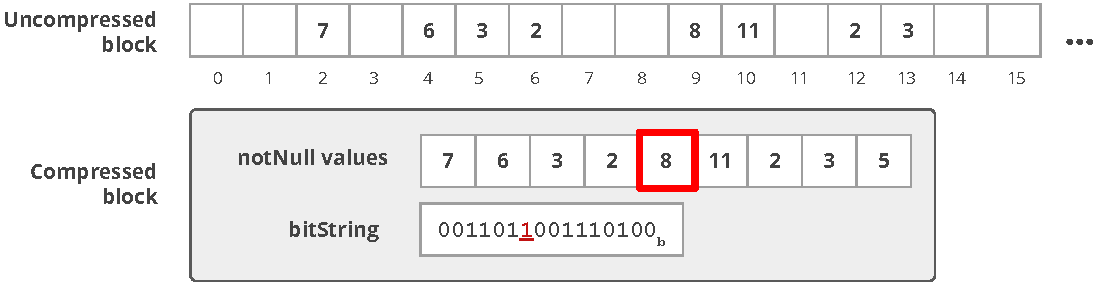
\includegraphics[scale=0.70]{img/null1}\hspace*{\fill}
	\captionsetup{justification=centering}
	\caption{\texttt{NULL} compression using bit-Strings.}
	\label{fig:null1}
\end{figure}

%The column is divided into block, where each compressed block holds 2 pieces of information: 1) a \textbf{non-\texttt{NULL}s array} that holds the non \texttt{NULL} values of the uncompressed block, and 2) a \textbf{bit-string} having a bit for each element in block, with 1's for non NULL elements. The storage overhead of the compressed block is only that of the bit-string which is 1 bit per element in the uncompressed block or 0.5 bit per non NULL element of the block that is 50\% occupied. Based on the sparsity, bit-string can be replaced by a list of offsets of non \texttt{NULL} elements in block for very sparse data, or list or ranges of non \texttt{NULL} elements for very dense data.

However, these techniques are not directly suitable for GDBMSs as they do not satisfy our Desideratum~\ref{des:compression}. In the bit-string method, we can in constant time learn whether or not if the value at a position $i$ is \texttt{NULL} or not (e.g., $i$ would be the positional offset of a vertex in a column storing a vertex property). However, if the value is not \texttt{NULL}, the system needs to iterate over the bits until location $i$ and count the number of $1$'s to find out the location of the value. For instance, in Figure~\ref{fig:null1}, accessing the element at index 9 of uncompressed block involves counting the number of 1's till before index 9 in the bit-string, which is 4. Thus, the value is then read from index 4 of the non-\texttt{NULL} values array. 

%Even though it is possible to operate on compressed column, the proposed scheme do not cater to our requirement of constant time random access. Reading from the compressed block involves iterating over the bit-string to calculate the location of the element in the non-\texttt{NULL}s array.

%\section{PrefixSum-based NULL Compression}
%\label{sec:prefixbased}

\begin{figure}
	\hfill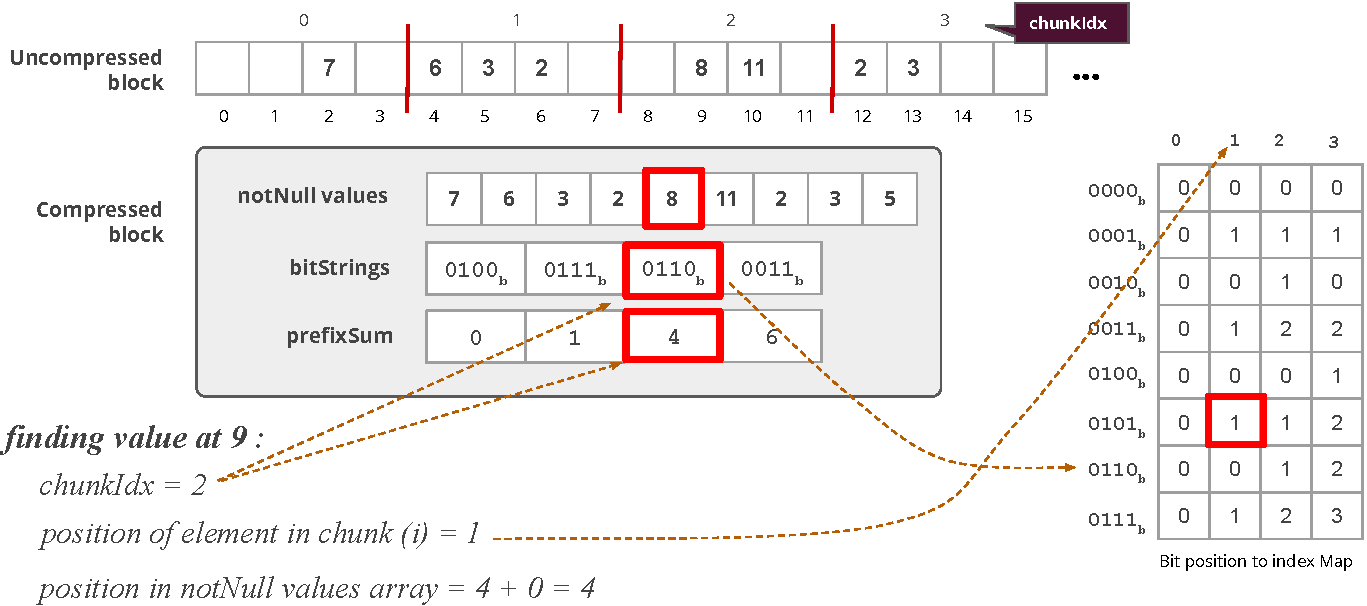
\includegraphics[scale=0.70]{img/null2}\hspace*{\fill}
	\captionsetup{justification=centering}
	\caption{PrefixSum-based \texttt{NULL} compression scheme. Chunk Size (n) = 4}
	\label{fig:null2}
\end{figure}

We next present a modification to the bit-string-based compression scheme to satisfy our requirement of constant time access to arbitrary elements. In addition to the array of non-\texttt{NULL} values and the bit-string, we store a prefixSum for each $c$ (16 by default) elements in a block of the column, i.e., we divide the block into chunks of size $c$. While the bit-strings indicate positions in the block with non \texttt{NULL} elements, the prefixSum holds the number of non \texttt{NULL} elements in the uncompressed block before a particular chunk. We also maintain a pre-populated static 2D map in the memory having size $(2^c, c)$. We call this \emph{bit-position-to-index map}. Let $b$ and $p$ respectively be the bit-string of length $c$ and prefixSum of a chunk $j$. Given $b$ and the position $i$ in the bit-string, the map returns the number of 1's in $b$ until position $i$. The map  allows us to avoid iterating over the bit-string to count the number of 1s and perform this count with a single lookup. Then, by adding the value returned from the map to $p$, we get the exact location of the value of location $i$ in $j$ (so the location of $j*c + i$ in the entire block). In total, after checking that the value is non-\texttt{NULL}, which needs to be done in any bit-string based scheme, we perform 1 lookup of prefix, 1 look up in the map, and 1 arithmetic, before the final look up of the actual value in the non-\texttt{NULL} values array.

%Therefore with 1 map lookup, 1 look1 arithmetic andFigure~\ref{fig:null2} depicts this prefix-sum-based null compression scheme. 

%We can directly to get the index of the element, at $i$ in the chunk, in the non-\texttt{NULL}s array. The index value returned by the map is relative to that chunk. This value, when added to $p$, gives the absolute index of the element, at $i$ in the chunk, in the non-\texttt{NULL} values array of the element.

% The prefixes at location $j$ indicates the total number of non-null values among the first $c*i$ locations in the column.  

%the solution to overcome the problem of constant time random reads in the existing solutions for compressing \texttt{NULL}s in sparse columns. The high-level idea is to do away with iteration over the bit-string while accessing the particular element in the compressed column.

%Figure~\ref{fig:null2} depicts compression of a sparse column using our scheme, which we call \emph{prefixSum-based null compression}. It divides a block into chunks of fixed size $n$. A compressed block contains 3 pieces of information: 1) a non-\texttt{NULL}s array, 2) an array of bit-strings and, 3) an array of prefixSums. We store one bit-string of length $n$ and a prefixSum per chuck. Whereas the bit-string indicates positions in the chunk with non \texttt{NULL} elements, the prefixSum holds the number of non \texttt{NULL} elements in the uncompressed block before the current block. 

Figure~\ref{fig:null2} depicts compression of a sparse column using our modified scheme. As an example, suppose we need to find the element at index 9 of the uncompressed block. Given $c=4$, this element will appear in the 2nd chunk, say $c_2$, of the compressed block. The position $i$ of index 9 in $c_2$ is 1. Also, $c_2$'s bit-string and prefixSum are $\texttt{0110}_b$ and 4 respectively. The entry for ($\texttt{0110}_b$, 1) in the bit-position-to-index map is 0. Thus, the index of element at 9 in non-\texttt{NULL} values array is $4+0 = 4$.

The choice of the value of $c$ affects how big the bit index to position map is. For $c = 16$, the size of the map is 1MB. The overhead of bit-string and prefixSum can also be optimized. Since the bit-string takes a bit for each element in an uncompressed block, the overhead depends on the size and number of prefixSums we have for an uncompressed block. By default we set $c$ to 16 and maintain blocks of size $N=2^c$ (so about 64K cells) and store our prefixSums as 16-bit unsigned integers. This ensures that the prefixes we keep increase the overhead from 1 to only 2 bits per element in the compressed block. If the size of prefixSum is $w$ and $c=16$, the overhead from prefixSums per element will be $w/16$ bytes. $w$ itself depends on the number of elements $N$ in the uncompressed block. For $N=2^{16}=64K$, $w=16$ and hence, the overhead of prefixSum is 1-bit per each cell in the block.

In our implementation, we use the prefix-sum based \texttt{NULL} compression schemes to compress vertex and edge properties (so vertex property columns and single-directional property pages) as well as empty lists in adjacency lists.  
%Our NULL compression scheme can be used orthogonally with any of the applicable columnar compression techniques that we discussed in section~\ref{sec:col-existing}. 
%We evaluate the effectiveness of our scheme in Chapter~\ref{c:evaluation} in effect to the storage savings by avoiding \texttt{NULL}s and the performance of queries when operating on \texttt{NULL} compressed columns.


















\chapter{List-based Query Processing}
\label{list-based-processing}

In this chapter, we introduce a new query processing technique, List-based query processing, for executing queries in a \gls{gdbms}. Our new processing technique benefits from orederly access of edges and its properties from the adjacency lists and edge property lists. Section~\ref{sec:existing-techniques} describes the different query execution models and lists the pros and cons for each of them. Next, we describe List-based processing in Section~\ref{sec:list-based-proc}

\section{Existing Techniques}
\label{sec:existing-techniques}
Almost all the \gls{gdbms} we are aware of uses the \textbf{Volcano-styled iteration model}~\cite{volcano} to execute a query. In the volcano-styled execution pipeline, each operator stores the reference of the next operators in the query plan. Execution happens tuple-at-a-time, with either operator operating on a partial match and pushing the result to the new operator in the pipeline. In particular, while processing a query volcano-styled, the edges of an adjacency list is read one at a time and processed further, making the access to the edge essentially random. Thus, this technique is oblivious to the fact that the edges in the adjacency lists are read in the same order in which they are stored, as stated in our Guideline~\ref{ssec:edges-ordered}. Clearly, processing the query volcano-styled does not agree with our Desiridatum~\ref{des1}. Even for the case of reading edge properties, we do not derive cache locality benefits from storing the properties of sequential edges nearby, since the access is mostly random. Also, the number of operations that are executed with volcano-styled processing is very high owing to the fact that each operator is particularly called as many times as there are input partial matches to. The large number of function calls adds significantly to the runtime of query execution on rad-intensive workloads.

\begin{example}
	\vspace{5pt}
	\label{ex:proc-example}
	Consider the following query. 
	{\em 
		\begin{lstlisting}[numbers=none,  showstringspaces=false,belowskip=0pt ]
		MATCH (a:PERSON)$-$[ex:FOLLOWS]$\rightarrow$(b:PERSON),
		$\qquad\quad$(b:PERSON)$-$[ey:FOLLOWS]$\rightarrow$(c:PERSON)
		WHERE a = $v4$
		RETURN ey.since\end{lstlisting}
	}
\end{example}
\vspace{-5pt}

\begin{figure}
	\hfill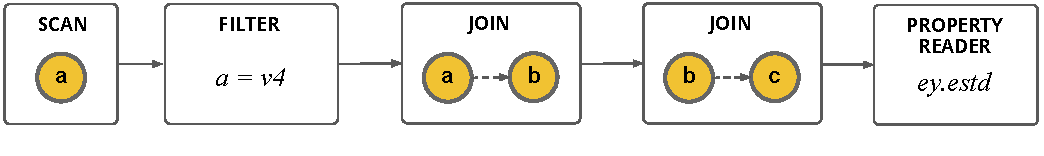
\includegraphics[scale=0.78]{img/proc-qp}\hfill
	\vspace{-10pt}
	\caption{Query plan for Example~\ref{ex:proc-example}.}
	\vspace{-8pt}
	\label{fig:proc-qp}
\end{figure}

Example~\ref{ex:proc-example} shows a 2-hop query starting from $v4$ of our example graph, while Figure~\ref{fig:proc-qp} shows a plan to execute the 2-hop query. In a volcano-styled processing-based system, this query is matches $a$ to $v4$ and $ex$ and $b$ respectively to the first element in $v4$'s adjacency list, i.e, $e2$ and $v1$. Next, $ey$ and $c$ is matched to the first edge in $v2$'s adjacency list, i.e. $e1$ and $v2$, before reading $e1$'s \texttt{since} property. Then, $ey$ is matched to $e9$ ($v2$'s second edge) and its property is returned. Now since $v2$'s adjacency list is exhausted, $ex$ is matched to second edge in $v4$'s adjacency list and processing continues. 

Alternative to volcano-styled iterator model is \textbf{column-at-a-time processing}~\cite{boncz-phd, monet-2decades} that is prevalent with columnar stors. While processing a column, this technique employs efficient block algorithms and tight loop over arrays that draw benefits from advanced compiler optimizations and even SIMD instructions in modern CPUs. Column-at-a-time processing can be applied to execute queries in \gls{gdbms}, in general, and to our solution, in particular, where it benefits from reading edges and its properties sequentially. The downside of operating column-at-a-time is the enormous amount of intermediary data that is produces with each operator that limits the execution in scalibility. This drawback is alleviated by yet another technique, called \textbf{Vectorized processing}~\cite{boncz-vectorwise1, boncz-monet-vectorized, boncz-vectorwise}, that proceses vector-at-a-time. Vectorized processing sits in beween the above two solution as it combines volcono-styled pipelineing with processing techniques of column-at-a-time processing. 

An intrinsic problem with operating vector-at-a-time or column-at-a-time is that of data duplication. The values of a vector gets duplicated each time an already matched vertex $v$ gets joined to an edge in $v$'s adjacency list. Hence, the duplication in query execution amplifies with each subsequent \texttt{JOIN}s in a query plan. Executing the query plan in Figure~\ref{fig:proc-qp} on example graph, the output of \texttt{SCAN(a)} is a single element vector $[v4]$. When \texttt{JOIN}ed with $b$, output is $[v4, e2, v1]$, $[v4, e5, v2], [v4, e3, v5]$, with $v4$ repeated in each. Joining with $c$ requires further duplication of $v4$ and its adjacent edges.

\section{List-based Processing}
\label{sec:list-based-proc}

A typical workload on a \gls{gdbms} involves matching long path queries on the input graph, which means a large number of usage of \texttt{JOIN} operators in the query plan. If such a query is executed in vectorized processing model, the problem of data duplication gets aggrevated to extreme levels and bulk of the query execution time is wasted in copying the input partial match. On the other hand, using pure volcano-style processing do not reap the benefits of ordered arrangement of data in adjacency lists and property pages. To elevate the problem of data duplication, we present a new query execution technique called \textbf{List-based processing}, that still uses the volcano-styles nesting of operators but processes a query by one adjacency list-at-a-time. In particular, a vertex $t$ in the partial match $t$ is joined to all adjacent edge and neighbour vertices in its adjacency list in a single execution of \texttt{JOIN} operator and are processed in a single operation by other operators like \texttt{PROPERTY READER} and \texttt{FILTER}. 

The implementation of List-based processing 














\chapter{Evaluation}
\label{c:evaluation}

We integrated our columnar storage and techniques into the in-memory GraphflowDB GDBMS. The version of the system we modified stored the edge and vertex properties in a row-oriented fashion as a sequence of variable-sized records indexed by their IDs and partitions the edges by labels and stores them as 8-byte vertex and edge IDs inside CSR. The goal of our experiments is two-fold. First, we show that using columnar storage and compression techniques reduces the memory consumption of the system significantly, by 3.5x, when storing a graph dataset generated by the popular LDBC social network benchmark. Second, we evaluate the query performance benefits and tradeoffs that these techniques provide. In particular, we organize our experiments as follows:
%  We show that redesigning the storage layer of \gls{gdbms} using columns that can harness the structure that exist in data  the graph can compact the storage by up to 3.5x.

\begin{enumerate}
	\item \textbf{Compression in Adjacency Lists:}  In Section~\ref{exp:adjacency-list-exp} we show the reduction in the size of our adjacency lists when applying the storage optimizations from Sections~\ref{c:columnar-storage} and~\ref{columnar-compression}. For each optimization, we state the cause of the reduction in size and query performance effect of the optimization.
		
	\item \textbf{Single-directional Property Pages:} In Section~\ref{exp:property-pages}, we compare the performance of storing edge properties in single-directional property pages, as compared to strictly-ordered single-directional property lists and unordered edge columns.
	
	\item \textbf{Vertex Columns for Single Cardinality Edges vs. CSR Adjacency Lists:}  In Section~\ref{exp:single-cardinality}, we show the effectiveness of storing single cardinality edges in vertex  columns as compared to in CSR format. 
	
	\item \textbf{Prefix Sum-based Null Compression:}  In Section~\ref{exp:prefixSum}, we evaluate the size  and performance tradeoff of compressing our columns with our prefix sum-based null compression scheme. We also compare our technique with the vanilla null compression technique mentioned in~\cite{abadi-sparse-col}.% to show the benefit of using a map instead of iterating over bit-strings.

	\item \textbf{List-based Processing vs Volcano-styled Query Execution:} In Section~\ref{exp:list-based}, we show the performance benefits of list-based processing over Volcano-styled processing.
	
\end{enumerate}

Noticeably missing in our evaluations is comparisons against the other \gls{gdbms} systems and conventional column stores, which we plan to perform as part of future work.

\section{Experimental Setup}

\noindent \textbf{Hardware Setup:} For all our experiments, we use a single machine that has two Intel E5-2670 @2.6GHz CPUs and 512 GB of RAM. The machine has 16 physical cores and 32 logical cores. We only use one logical core. We set the maximum size of the JVM heap to 500 GB and keep JVM's default minimum size.

\begin{figure}
	\centering
	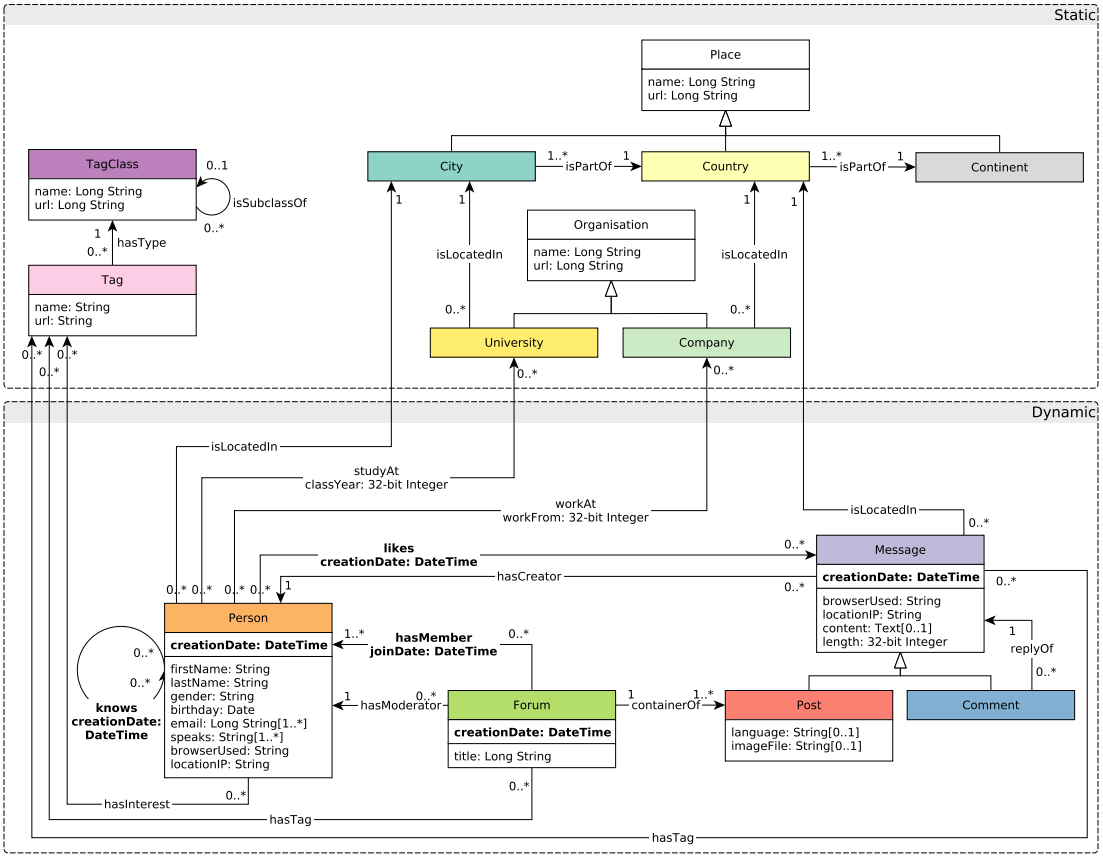
\includegraphics[scale=0.42]{img/ldbc-schema}
	\captionsetup{justification=centering}
	\caption{\gls{ldbc} Graph schema. (Obtained from LDBC SNB specification document v0.3.2)}
	\label{fig:ldbc-schema}
\end{figure}

\noindent \textbf{Dataset:} We use the \gls{ldbc}~\cite{ldbc} dataset generator to generate synthetic graph datasets on which we evaluate all our experiments. \gls{ldbc} is a popular benchmark to generate large social graph data with attributes on nodes and edges. The generated social graph is highly structured which can be seen from the schema in Figure~\ref{fig:ldbc-schema}. In fact all of the edges and edge and vertex properties are structured according to our definition from Chapter~\ref{c:guidelines} but several properties and edges are very sparse. For example, property X on vertices with type X appears in less than X\% of the nodes with type X.\todo{Complete the X's.}  We generate the data at the scale factor of 100 (LDBC100) that consists of over 1.7 billion edges and 0.3 billion vertices. We refer to this dataset as LDBC100

\noindent \textbf{Query Workload:} We use a micro benchmark we generate that consists of 1-, 2-, and 3-hop path queries that optionally contain predicates on vertex and edge properties and aggregations. These queries serve as a stress test for evaluating access to the underlying storage, which our techniques optimize. 
%For instance, a simple 1-hop query tests more rigorously for access from adjacency lists than a query that involves filtering and aggregations. 

\section{Compression in Adjacency Lists}
\label{exp:adjacency-list-exp}

%We introduced several optimizations that can make use of the graph data's structure to drastically compact the representation of edges and vertices in the adjacency lists. 
In this experiment, we demonstrate the memory reduction we get from the columnar storage and compression techniques we described in this thesis that reduce the cost of storing (edgeID, neighborID) pairs in adjacency lists.% that exploits structure in graph data on LDBC100.  
% optimizations on LDBC100 by recording the memory utilization of the adjacency lists across different %configurations which we describe momentarily.
We create multiple configurations on GraphflowDB, each with a different set of optimizations. Below are the descriptions of the configurations we evaluate the memory usage on. Each configuration builds on top of previous in the list. 

\begin{enumerate}
	\item \texttt{GF-OLD:} This is our baseline configuration that represents edges and vertices in the adjacency list as 8-byte identifiers. All the edges are stored in the 2-level CSR structure and are not compressed.
	\item \texttt{+COLS}: Uses vertex columns from single cardinality edge labels. 
	\item \texttt{+NEW-IDS}: Introduces our new vertex and edge identification schemes.
	\item \texttt{+0-SUPR}: Implements leading 0 suppression in the components of vertex and edge IDs in adjacency lists.
	\item \texttt{+OMIT}: Omits neighbor vertex label and positional offsets of edge IDs when they can be inferred from the structure.
	\item \texttt{+NULL}: Implements prefix sum-based null compression on adjacency lists (or vertex columns for single cardinality edges).
\end{enumerate}

\begin{table}
	\centering
	\bgroup
	\setlength{\tabcolsep}{8pt}
	\def\arraystretch{1.2}%  1 is the default, change whatever you need
	\begin{tabular}{ |c|c|c|c|c|c|c| } 
		\hline
		& \texttt{GF-OLD} & \texttt{+COLS} & \texttt{+NEW-IDS} & \texttt{+0-CMPRS} & \texttt{+OMIT}& \texttt{+NULL} \\ 
		\hline \hline
		\multirow{2}{120pt}{Fwd. Adjacency Lists}& 38.25 & 33.25 & 27.22 & 16.35 & 11.14 & 10.53 \\ 
		& & \textbf{+1.15x} & \textbf{+1.22x} & \textbf{+1.66x} & \textbf{+1.47x} & \textbf{+1.06x} \\ 
		\hline
		\multirow{2}{120pt}{Bwd. Adjacency Lists}& 37.93 & 37.50 & 30.93 & 18.75 & 12.79 & 11.15 \\ 
		& & \textbf{+1.01x} & \textbf{+1.21x} & \textbf{+1.65x} & \textbf{+1.47x} & \textbf{+1.15x} \\ 
		\hline
		\multirow{3}{120pt}{Total (GB)\\Bytes Per Edge\\} & 76.18 & 70.75 & 58.15 & 35.10 & 23.93 & 21.68 \\ 
		 & 23.04 & 21.39 & 17.58 & 10.61 & 7.24 & 6.50 \\ 
                 & & \textbf{1.08x} & \textbf{1.31x} & \textbf{2.17x} & \textbf{3.18x} & \textbf{3.55x} \\  
%		\hline \hline
%		\multirow{3}{80pt}{Bytes per edge}& 23.04 & 21.39 & 17.58 & 10.61 & 7.24 & 6.50 \\ 
%		& & \textbf{1.08x} & \textbf{1.31x} & \textbf{2.17x} & \textbf{3.18x} & \textbf{3.55x} \\ 
		\hline
	\end{tabular}
	\egroup
	\captionsetup{justification=centering}
	\caption{Memory utilization (in GB) by Adjacency lists of  LDBC100 when adding our optimizations one at a time. Each column $i$ indicates an optimization $i$ and in the rows for forward and backward lists indicate the additional reduction factor of applying optimization $i$ on top of the previous optimizations to the left of $i$. In contrast, in the row on total memory consumption/bytes per edge, each column $i$ indicates the cumulative reduction factor (compared to \texttt{GF-OLD}) of applying all optimizations from left until $i$.}
	\label{tbl:mem1}
\end{table}

\begin{figure}
	\centering
	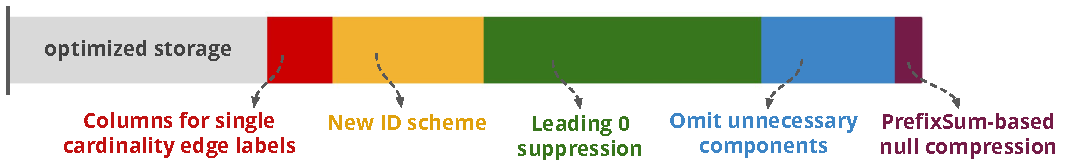
\includegraphics[scale=0.75]{img/opti-breakup}
	\captionsetup{justification=centering}
	\caption{Breakup of memory gains by applying different optimizations on Adjacency Lists of \gls{ldbc} scale factor 100 dataset.}
	\label{fig:opti-breakup}
\end{figure}

Table~\ref{tbl:mem1} shows how much memory (in GB) the adjacency lists take when storing the edges of LDBC100 across different configurations.  Figure~\ref{fig:opti-breakup} gives the breakup of memory gain per optimization. Memory gain in \texttt{+COLS} is attributed to the fact that 8 out of 15 edge labels are single cardinality and stored in vertex columns in at least one direction. \texttt{+NEW-IDS} gains ({\raise.17ex\hbox{$\scriptstyle\sim$}}4 bytes per edge) by storing edges in smaller than 8 bytes, while \texttt{+OMIT} gains ({\raise.17ex\hbox{$\scriptstyle\sim$}}3 bytes per edge) from not storing edge's positional offsets and neighbour's vertex label for 10 out of 15 edge labels. We see modest benefits in \texttt{+NULL} ({\raise.17ex\hbox{$\scriptstyle\sim$}}0.75 bytes per edge) since empty adjacency lists are infrequent in LDBC100.

All of these optimizations also improve query performance, with the exception of \texttt{+NULL}, which incurs a modest query slow down. We will evaluate the performance gains and tradeoffs of \texttt{+COLS} and \texttt{+NULL} are evaluated in Sections~\ref{exp:single-cardinality} and ~\ref{exp:prefixSum} respectively. 
We will not evaluate the benefits of leading 0 suppression but we note that this also improves performance because we do not have to decode a particular value and hence, and have modest gains because we copy less data into tuples from the adjacency lists.

%Further, the memory utilization of \gls{ldbc} 300 (5.27B edges, 0.6B vertices) with our set of optimizations was 63.45GB. In all, we are able to scale the new GraphflowDB (with our new storage layer) to store up to 10.5B edges, along with vertex and edge properties, of \gls{ldbc} data on a single machine with 500GB of main memory. This is {\raise.17ex\hbox{$\scriptstyle\sim$}}15x increase in scalability compared to old GraphflowDB with unoptimized storage.

\section{Effectiveness of Single-Directional Property Pages}
\label{exp:property-pages}

In this experiment, we show the benefits of keeping the edge properties grouped in single-directional property pages compared to using edge columns that store the edge properties in an unordered way. 
Recall that one alternative design we described was using  single-directional property lists to store edge properties. This design had the advantage that edge properties would be kept in exactly the same order as they appear in adjacency lists, but it can make updates significantly slower, specifically for systems that keep edges in sorted order. However, this design may still be a viable design for some GDBMSs and as a point of reference we also evaluate its benefits. 
%We also demonstrate that keeping edge properties in property pages instead of single-directional property lists is a reasonable trade-off as we lose modest performance. but significantly win over edge columns. 
To test the performance benefits of single-directional property pages and lists, we configure GraphflowDB  in 3 different ways (all using our new ID schemes):

\begin{enumerate}
	\item \texttt{EDGE COLS:} Stores edge properties in edge column in the order they were inserted into the database, so properties of edges in a particular adjacency list (forward or backward) can appear anywhere in this column. We ensure that the insertion order is random. % in  If there are $|E|$ many e For example, the edge properties of label \texttt{knows} are stored in columns that are oblivious to the location of \texttt{knows} edges in either the forward or backward adjacency lists. 
	\item \texttt{PROP LISTS:} Edge properties are stored in the single-directional property lists. We pick the forward list for $n-n$ multiplicity edges. Therefore these property lists mimic the forward adjacency lists and gives sequential reads when edge properties of a forward adjacency list are read.
	
	\item \texttt{PROP PAGES:} Edge properties are stored in pages by combining $n=128$ property lists of the previous solution and appear in insertion order. This solution provides close-by reads when edge properties of a forward adjacency list are read.
\end{enumerate}

\begin{table}
	\centering
	\bgroup
	\setlength{\tabcolsep}{8pt}
	\def\arraystretch{1.2}%  1 is the default, change whatever you need
	\begin{tabular}{ |c|c|c|c| } 
		\hline
		& \textbf{1-hop} & \textbf{2-hop} & \textbf{3-hop} \\
		\hline \hline
		\texttt{EDGE COLS}& 3.42 & 308.18 & 966.04\\ 
		\hline 
		\multirow{2}{*}{\texttt{PROP PAGES}} & 1.22 & 152.89 & 512.24 \\ 
		& \textbf{2.80x} & \textbf{2.03x} & \textbf{1.87} \\ 
		\hline
		\multirow{2}{*}{\texttt{PROP LISTS}}& 1.03 & 125.65 & 372.44 \\ 
		& \textbf{3.32x} & \textbf{2.42x} & \textbf{2.59}\\ 
%		\hline \hline
%		\texttt{PROP PAGES} vs \texttt{PROP LISTS} & 1.19x & 1.22x & 1.37x \\
		\hline
	\end{tabular}
	\egroup
	\captionsetup{justification=centering}
	\caption{Runtime (in sec) of k-hop queries for different configurations of edge property storage on LDBC100.}
	\label{tbl:mem2}
\end{table}

As our workload, we use 1- 2- and 3-hop queries that use the \texttt{knows} edge label of the \gls{ldbc} schema (Figure~\ref{fig:ldbc-schema}) that compare each query edge's \texttt{creationDate} property to be greater than the previous edge's. 1-hop and 2-hop queries run for all vertices of \texttt{person} while we run 3-hop for only 25000 vertices to make the queries faster. For each query, we only consider the plan that matches vertices from left to right in the forward direction. This way, we are ensure cache locality for \texttt{PROP-LISTS} and \texttt{PROP-PAGES}. Table~\ref{tbl:mem2} shows the performance of queries on 3 configurations. We observe that the queries benefit significantly from localizing edge properties in the storage. Compared to \texttt{EDGE COLS}, we see up to 2.8x improvement for \texttt{PROP PAGES} and up to 3.32x improvements for \texttt{PROP LISTS}. Recall also that using \texttt{PROP PAGES} or \texttt{PROP LISTS} also reduces our storage because the amount of bytes required to identify edges within a list or a property page is smaller than the bytes needed to identify an edge within an entire edge column. In a system that uses fixed size IDs, which in-memory systems optimized for performance should do, 8 bytes is needed to identify edges in billion-scale graphs while 4 bytes is sufficient to identify edges within a list or property page. Finally, note that the benefits we get from \texttt{PROP PAGES} will depend on $n$, in particular as $n$ approaches 1, \texttt{PROP PAGES} design reduces to \texttt{PROP LISTS}. We have not performed this experiment but as $n$ gets smaller we expect the performance differences between \texttt{PROP LISTS} and \texttt{PROP PAGES} to reduce.

% In addition, using property lists or pages allows us to use positional offsets that need to identify edges within a list of a property page (so 128 lists). 
%The benefits decrease with the size of query because the last operators in a query plan flush the pages from which earlier operators read. However, both property lists and pages still guarantee benefits over unordered \texttt{EDGE COLS}. On the other hand, storing the edge properties in the update-friendly property pages only slightly degrades the performance of queries (1.19-1.37x). This depends on the value of $n$, i.e, the number of property lists that we put together on a page. The average number of \texttt{knows} edges per \texttt{person} vertex is {\raise.17ex\hbox{$\scriptstyle\sim$}}44 edges while $n=128$. A lower $n$ means that properties of edges in an adjacency lists appear closer in the page and hence, provide more localized reads.

\section{Vertex Columns for Single Cardinality Edges vs CSR Adjacency Lists}
\label{exp:single-cardinality}

Storing single cardinality edges in vertex columns ensure two benefits: (i) direct access into the edge without indirection into CSR, and 2) does not need to store offsets of the CSR. We showed the memory gains of storing edges in vertex columns in Section~\ref{exp:adjacency-list-exp}. We next compare the performance benefits of using vertex column vs adjacency lists in CSR format under two settings: (i) when empty lists (or edges because of single cardinality) are not null compressed; and (ii) when they are null compressed. We create 4 configurations of GraphflowDB to run our queries on:

\begin{enumerate}
	\item \texttt{V-COL-UNC:} Single cardinality edge label edges are stored in vertex columns and are not compressed. 
	\item \texttt{CSR-UNC:} Single cardinality edge label edges are stored in CSR format and are not compressed.
	\item \texttt{V-COL-C:} Null compressed version of \texttt{V-COL-UNC}. This is equivalent to \texttt{+NULL} configuration in Section~\ref{exp:adjacency-list-exp}.
	\item \texttt{CSR-C:} Null compressed version of \texttt{CSR-UNC}.
\end{enumerate}

The workload consists of simple 1-, 2-, and 3-hop queries on the \texttt{replyOf} edge between \texttt{comment} vertices in the \gls{ldbc} schema. The \texttt{replyOf} edge label has \texttt{n-1} cardinality, hence, we keep the forward edges as a special property of \texttt{comment} vertex label. Moreover, our workload queries do not do any predicate evaluation and the final output of the query is an aggregated count. This assures that \texttt{JOIN} operation in the query plan is the only dominant operation. Again, for each query, we evaluate only on the plan that matches the vertices sequentially and joins in the forward direction.

\begin{table}
	\centering
	\begin{subtable}{1\textwidth}
		\centering
		\bgroup
		\setlength{\tabcolsep}{8pt}
		\def\arraystretch{1.2}%  1 is the default, change whatever you need
		\begin{tabular}{ |c|c|c|c|c| }
			\hline
			& \textbf{1-hop} & \textbf{2-hop} & \textbf{3-hop} & \textbf{Memory (in MB)} \\ 
			\hline \hline
			\texttt{CSR-UNC}& 7.03 & 9.13 & 9.60 & 1266.56 \\ 
			\hline
			\multirow{2}{*}{\texttt{V-COL-UNC}}& 4.34 & 5.80 & 5.85 & 839.93 \\ 
			& \textbf{1.62x} & \textbf{1.57x} & \textbf{1.64x} & \textbf{1.51x} \\ 
			\hline
		\end{tabular}
		\egroup
		\captionsetup{justification=centering}
		\caption{Uncompressed}
		\label{tbl:s1}
	\end{subtable}
	\begin{subtable}{1\textwidth}
		\centering
		\bgroup
		\setlength{\tabcolsep}{8pt}
		\def\arraystretch{1.2}
		\begin{tabular}{ |c|c|c|c|c| } 
			\hline
			& \textbf{1-hop} & \textbf{2-hop} & \textbf{3-hop} & \textbf{Memory (in MB)} \\ 
			\hline \hline
			\texttt{CSR-C}& 7.78 & 10.40 & 11.23 & 905.23 \\ 
			\hline
			\multirow{2}{*}{\texttt{V-COL-C}}& 5.23 & 8.28 & 8.41 & 478.86 \\ 
			& \textbf{1.49x} & \textbf{1.26x} & \textbf{1.34x} & \textbf{1.89x} \\ 
			\hline
		\end{tabular}
		\egroup
		\captionsetup{justification=centering}
		\caption{Null Compressed}
		\label{tbl:s2}
	\end{subtable}
	\captionsetup{justification=centering}
	\caption{Vertex property columns vs. 2-level CSR adjacency lists for storing single cardinality edges: Query runtime (in sec) and Memory usage (in MB)  }
\end{table}

Tables~\ref{tbl:s1} and ~\ref{tbl:s2} shows the result of queries on uncompressed and null compressed configurations respectively. We observe up to 1.62x performance gains between uncompressed variants of vertex columns and CSR (i.e., \texttt{V-COL-UNC} vs \texttt{CSR-UNC}) and up to 1.49x gains between null compressed variants (i.e.,  \texttt{V-COL-C} vs \texttt{CSR-C}). The last column of the tables report the size of the adjacency lists or vertex column storing \texttt{replyOf} edges. Here, vertex column uses half as much space as adjacency lists, when the data is kept compressed. In LDBC100, out of {\raise.17ex\hbox{$\scriptstyle\sim$}}220M \texttt{comment} vertices 50.5\% have empty forward adjacency list, i.e, do not have an outward \texttt{replyOf} edge. This is reflected in vertex columns between \texttt{V-COL-UNC} and \texttt{V-COL-C}, as the memory reduces by 1.75x (839.93MB vs 478.86MB), unlike their CSR counterparts that stores offsets as extra and thus, compression reduces memory by only 1.4x (1266.56 vs 905.23). These results verify that using vertex columns for single-cardinality edges not only saves space, but also improves query performance (irrespective of whether or not the edges/lists are null compressed or not).

\section{Effectiveness of Prefix Sum-based Null Compression}
\label{exp:prefixSum}

We demonstrate the memory performance tradeoff of prefix sum-based null compression when compressing both sparse property columns as well as empty adjacency lists. We evaluate two aspects of our technique: (i) storage and random access efficacy against uncompressed and vanilla null compressed columns; and (ii) query performance on compressed and uncompressed vertex columns and adjacency lists.

%\subsection{Stress Test} 

\begin{figure}
	\hspace*{-25pt}
	\begin{subfigure}{0.55\textwidth}
		\centering
		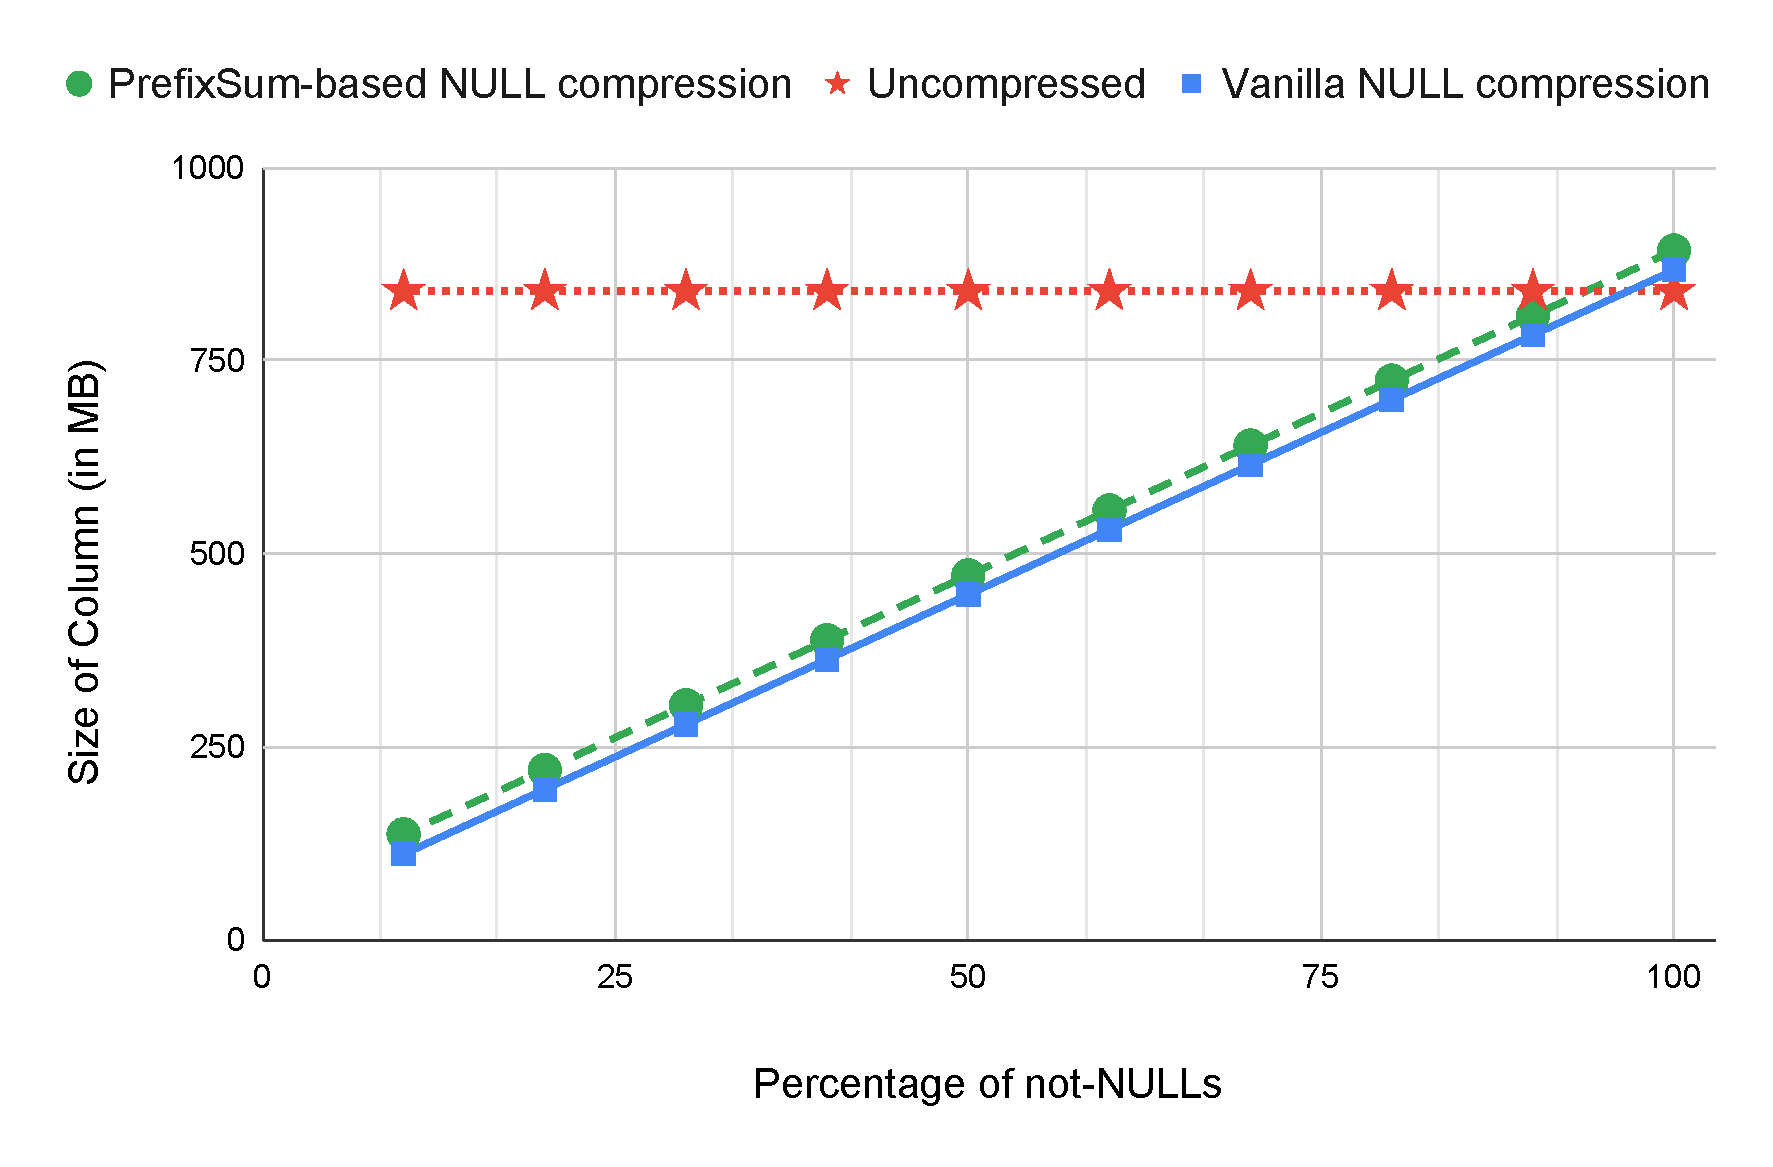
\includegraphics[scale=0.30]{img/pref-space}
		\captionsetup{justification=centering}
		\caption{Memory usage}
		\label{fig:pref-space}
	\end{subfigure}
	\begin{subfigure}{0.55\textwidth}
		\centering
		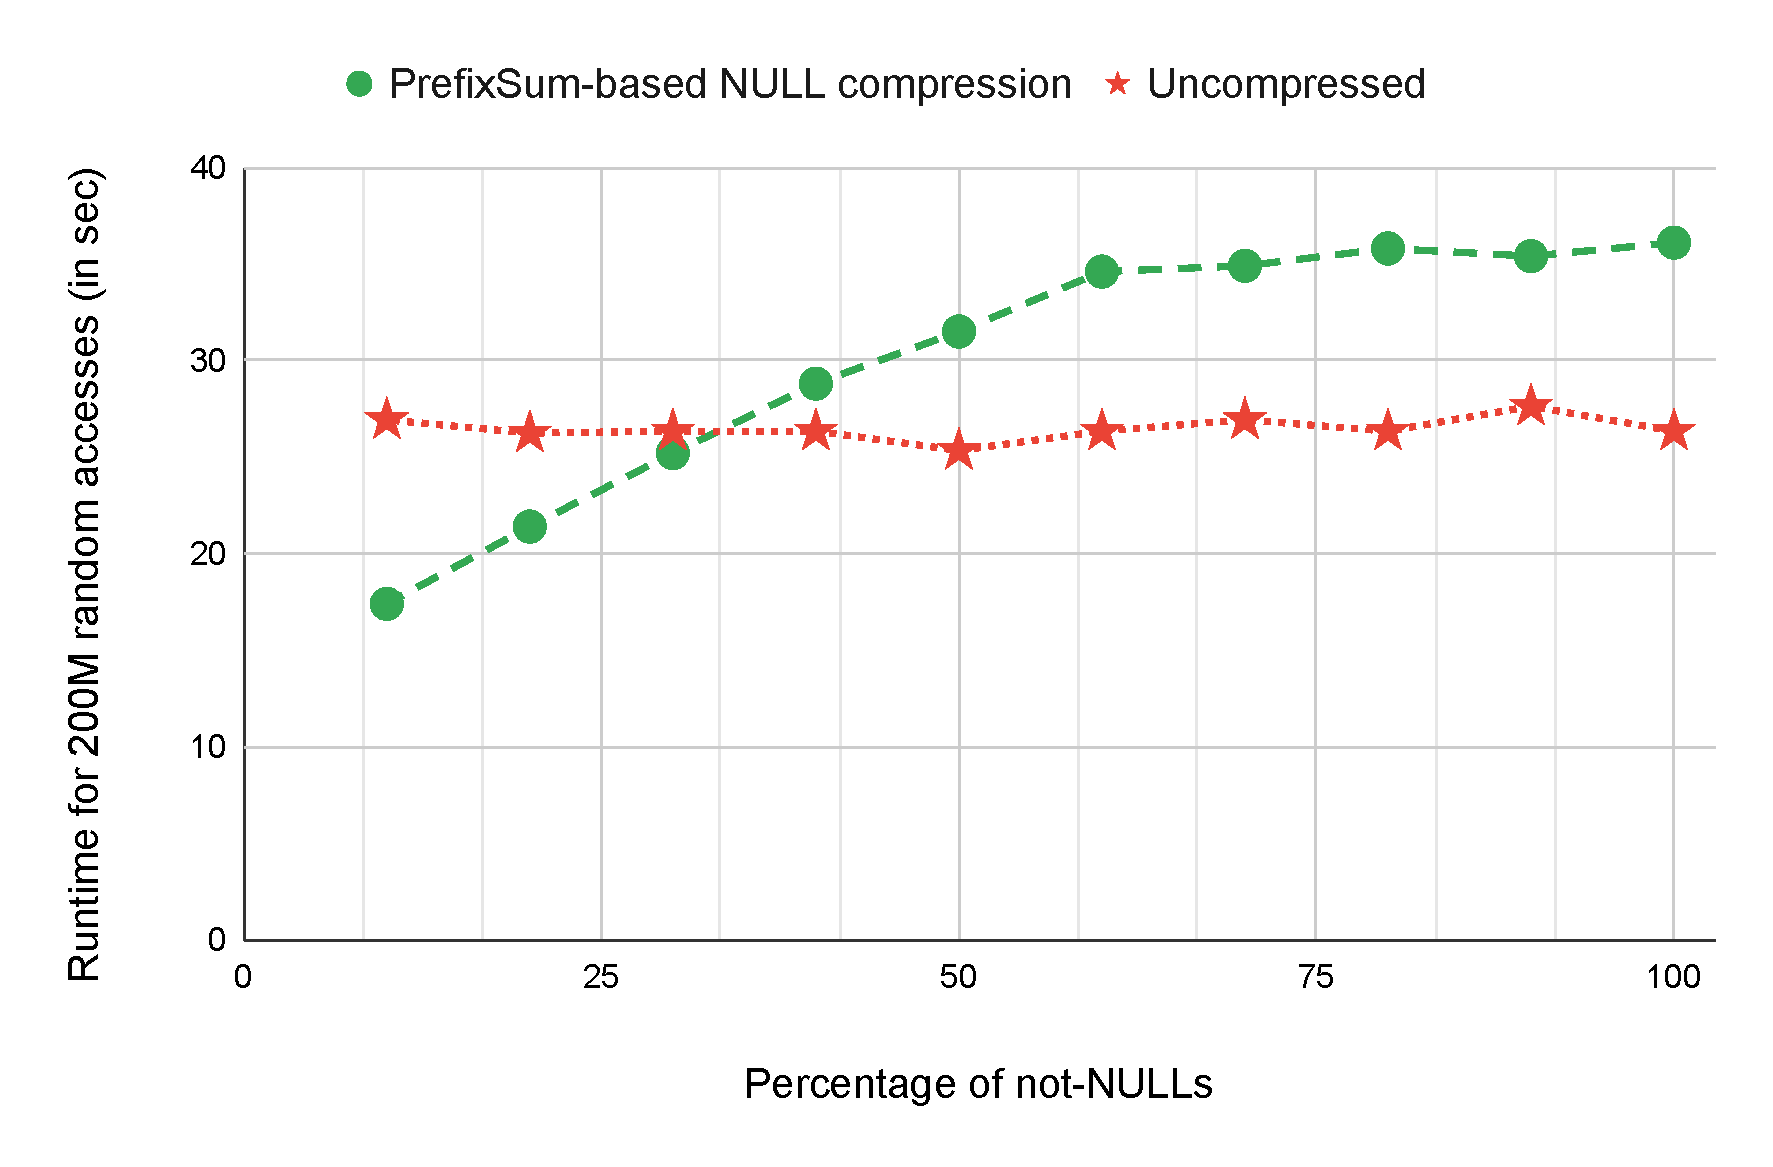
\includegraphics[scale=0.30]{img/pref-perf}
		\captionsetup{justification=centering}
		\caption{Performance on random accesses}
		\label{fig:pref-perf}
	\end{subfigure}
	\captionsetup{justification=centering}
	\caption{Memory and performance on random accesses for Uncompressed, prefix sum-based NULL compressed and vanilla NULL compressed columns.}
	\label{fig:pref-stress}
\end{figure}

The goal of our first experiment is to compare uncompressed, prefix sum-based null compressed and vanilla null compressed (as implemented in ~\cite{abadi-sparse-col}) columnar data-structure for memory usage and performance on random reads. We design a micro-benchmark to stress test the access performance when performing random accesses to a null compressed column. We use the \texttt{creationDate} property of 220M \texttt{comment} vertices in LDBC100 and create multiple versions of it, each with different percentage of non-null values. On each version, we do the necessary compression and measure the time taken to do 200M access to random locations in the column. 

Figures~\ref{fig:pref-space} and~\ref{fig:pref-perf} show memory usage and performance on 200M random read queries respectively, for uncompressed, prefix sum-based null compressed and vanilla null compressed column of \texttt{creationDate} property of \texttt{comment} vertex label. We omit the performance number of vanilla null compression as they were significantly higher than the other two configurations ($>$20x). Our prefix sum-based  compression technique requires slightly more memory than vanilla null compression technique (2-bit for each element vs. 1-bit overhead in vanilla compression). However, introducing prefix sums and map lookups in stead of iterations over bit-strings of each block provide significant performance benefits. We observe at most 1.38x slow down the performance compared to the uncompressed column, which has no decompression cost. Surprisingly, accesses in prefix-sum based compression can even be faster than accesses to an uncompressed column when the column is very sparse ($<30\%$ non-null values). This is because testing for null at a location is a constant time operation and when most of the accesses return null, in a null compressed column, the iterators return a single global variable that keeps  the null value for the data type. Instead, in an uncompressed column, the null value from the column is copied, which has a higher chance of a CPU cache miss. 

%\subsection{Query Performance}

Tables~\ref{tbl:s1} and~\ref{tbl:s2} already compares reading edges from compressed and uncompressed adjacency lists and vertex columns. Reading edges from CSR adjacency lists and vertex columns that are null compressed by our technique are on average 1.14x and 1.3x slower than their uncompressed variant respectively. However, for 50\% null values, they gain 50\% and 25\% in storage respectively. 

\begin{table}
	\centering
	\bgroup
	\setlength{\tabcolsep}{8pt}
	\def\arraystretch{1.2}%  1 is the default, change whatever you need
	\begin{tabular}{ |c|c|c|c| } 
		\hline
		& \textbf{1-hop} & \textbf{2-hop} & \textbf{3-hop} \\
		\hline \hline
		\texttt{V-COL-UNC}& 12.78 & 14.47 & 14.95\\ 
		\hline
		\multirow{2}{*}{\texttt{V-COL-C}}& 14.65 & 16.00 & 16.98 \\ 
		& \textbf{1.15x} & \textbf{1.11x} & \textbf{1.14x}\\ 
		\hline  
	\end{tabular}
	\egroup
	\captionsetup{justification=centering}
	\caption{Runtime (in sec) of k-hop queries on compressed and uncompressed vertex column on LDBC100.}
	\label{tbl:s3}
\end{table}

In our second experiment, we evaluate accessing vertex properties from compressed and uncompressed vertex columns using k-hop queries. We use the \texttt{V-COL-C} and \texttt{V-COL-UNC} configurations and keep the edge storage uncompressed. We run the workload from Section~\ref{exp:single-cardinality} consisting of k-hop queries over \texttt{replyOf} edges. These queries are extended to include a condition that a \texttt{comment} $b$ is made on another \texttt{comment} $a$ such that $b$ has a \texttt{creationDate} that is within $\delta$ timespan of $a$'s. Table~\ref{tbl:s3} shows our results. Using compressed storage slows down our queries by at most 1.14x. Therefore compared to the vanilla null compression schemes, which are not practical, our prefix sum-based null compression scheme is a practical compression scheme that offers a good performance and memory trade-off.

\section{List-based Processing vs. Volcano-styled Query Execution}
\label{exp:list-based}

We compare list-based query processing to the conventional volcano-styled processing on several path queries.























\chapter{Related Work}
\label{c:related-works}

This thesis studied the integration of columnar storage and query processing techniques to GDBMSs. We review related work on column-oriented relational systems and other storage and compression techniques that have been designed for GDBMSs and RDF engines. There is an extensive literature on different storage and compression techniques designed for specific graphs, which we do not cover here. We refer the interested readers to reference \cite{sahu:survey, besta2018survey} for a survey on the lossless compression techniques from literature. These techniques focus on compressing the topology of the graph and broadly can achieve high compression rates for special types of graphs, e.g., Erd\H{o}s R\'enyi graphs or web graphs, but require decompression while accessing adjacencies. Therefore they are less applicable for an in-memory GDBMS that the techniques we considered in this thesis.

% on columnar storage and compression for GDBMSs and graph query processing. Section~\ref{graph-compression} discusses works in representing graphs and graph databases for a number of use cases. Section~\ref{column-storage} talks about existing solutions employing columnar storage and compression in \gls{rdbms} and RDF databaes. 

\section{Storage and Compression Techniques in Column-Oriented Relational Systems}
\label{sec:column-stores-overview}

Column-oriented RDBMSs are designed primarily for OLAP applications that are analytics heavy that perform aggregations over entire tables or subsets of tuples. At a high-level these systems store the relations in disk pages as a set of separate columns, instead of a set of rows. The column $c$ value of a particular row $r$ can be found using a positional offset, using the row ID of $r$, in the page that stores column $c$. The row IDs are referred to as surrogate keys. Prior to the emergence of column stores, such as C-Store~\cite{c-store}, MonetDB~\cite{monet-2decades}, and VectorWise~\cite{boncz-vectorwise, boncz-vectorwise1},  prior work, such as PAX~\cite{pax}, had used columnar storage inside in the context of row-oriented systems. PAX was a storage design that stores a set of rows in each disk page, but organizes the rows inside each page in a columnar format. 

Many prior work on column stores introduced a set of columnar storage, compression, and query processing techniques. These techniques include: positional offsets (also called virtual IDs) to directly access values in columns for different rows, columnar compression schemes, vector-oriented query processing, late materialization, and direct operation on compressed data among others. A detailed survey of these techniques can be found in reference~\cite{design-imp-book}, which reviews the techniques introduced in C-Store, MonetDB, and VectorWise.  This thesis studied how to directly integrate these techniques to in-memory GDBMSs or modify and adapt them so that they can be integrated into in-memory GDBMSs. The most relevant techniques that we identified and integrated are:  (i) a set of columnar storage structures to store different components of property graphs (shown in Table~\ref{tbl:summ}); (ii) vertex and edge ID schemes that allow direct positional offsets into these columns; (iii) compression schemes that include dictionary encoding, zero suppression, compressed edge and vertex IDs, and a null and empty-list compression scheme;  and (iv) list-based processing which is a hybrid between Volcano-style and vector-oriented processing. 

For disk-based GDBMSs, other techniques, in particular other compression schemes, such as run-length encoding to compress vertex and edge properties, or integer compression schemes from reference~\cite{lemire:integer} to compress adjacency lists might also be beneficial. For an in-memory systems these techniques can increase the systems scalability but they will also decrease performance as data needs to be decompressed before accessing. Except for null-compression, our other compression schemes do not decrease an in-memory \gls{gdbms}'s performance as they do not require decompression. Null compression slows down query execution but not significantly, so offers a good performance and space trade-off. Whether or not \gls{gdbms}-specific versions of other compression schemes can be developed for in-memory GDBMSs is an interesting research direction.

% are known to have their own set of optimizations and processing techniques that makes it highly efficient in storage and processing, like block processing, compression etc. \cite{col-vs-row, design-imp-book}. C-Store \cite{c-store} is an updatable column storage system that keeps multiple copies of columns sorted differently and uses positional offsets in a column to process data. Building on it, \cite{abadi-col-comp, abadi-sparse-col} talks about light-weight compression and execution over compressed data in C-Store. MonetDB \cite{monet-2decades} assumes similar vertical partitioning into columns \texttt{(BAT)} but follows a different execution stratetegy by means of binary opeations on BAT. MonetDB benefits from tight for-loops and bulk processing that give then good cache locality and avoids instruction misses. Even though our idea of vertical partitioning is in line with these works, our solution is native for \gls{gdbms} and hence organizes and executes process differently.

\section{Storage and Compression for GDBMSs and RDF Systems}
\label{sec:gdbms-storage-and-compression}

There are several existing native GDBMSs, whose internals have been described in technical papers or documents. These systems adopt a columnar structure only for storing the topology of the graph. This is done either by using a variant of vanilla adjacency list format or CSR. These systems use other row-oriented structures, such as property stores that store a sequence of key-value properties, or a separate key-value store to store vertex and edge properties. For example, Neo4j~\cite{neo4j} represents the topology of the graph in adjacency lists that are partitioned by edge labels and stored in linked-lists, where each edge record points to the next that is not necessarily stored consecutively in disk. Similarly, the property of each vertex and edge are stored in a linked-list in an unstructured manner, where each property record points to the next property record and encodes the key, data type, and value of the property. This can be seen as adopting a row-oriented storage for properties. Similarly, JanusGraph \cite{janusgraph} stores its edges in adjacency lists partitioned by edge labels and properties as a consecutive key-value pairs (so in row-oriented format). JanusGraph uses variable-length encoding when storing edges in the adjacency lists. Instead, we use fixed-length encodings in our compression schemes. DGraph~\cite{dgraph} uses key-value store to hold adjacency lists as well as properties.  We are unaware of any compression schemes adopted by Neo4j and DGraph. All of the above native GDBMSs adopt Volcano-style processors. In contrast, our design adopts columnar structures for vertex and edge properties and a list-based processor. Our storage techniques and list-based processing allows our system to benefit more from data locality. In addition we improve on these designs by more compressed edge and vertex ID representation (these systems use 8 bytes for each ID) and null compression.

There are also several GDBMSs that are developed directly on top of an RDBMS or another database system. For example Oracle Spatial and Graph~\cite{oracle} supports a property graph model using the PGQL language~\cite{pgql} that is built on top of Oracle database. SAP's graph database~\cite{hana-graph} is developed on top of HANA. These systems can benefit from the columnar techniques provided by the underlying RDBMS but the underlying RDBMS techniques are not optimized for graph storage and queries. For example, SAP's graph engine uses SAP HANA's columnar-storage to store vertex and edge tables but these columns do not have CSR-like structures for indexing edges of each vertex. Similarly existing RDBMSs do not implement null compression schemes similar to our prefix-sum-based scheme that allow constant-time access to arbitrary column values.

RedisGraph~\cite{redisgraph} is a system that stores its adjacency lists and properties inside the Redis~\cite{redis}, a distributed in-memory key value database. Though RedisGraph's latest release we are aware of runs only in single nodes. RedisGraph has a query processor that is based on performing linear algebra operations. The system converts Cypher queries into a sequence of linear-algebra based operators, which are executed using the GraphBLAS~\cite{graphblas} linear algebra library. This can be seen as performing column-oriented processing, as entire columns, which are stored in, are processed during query evaluation. We have not benchmarked our system against RedisGraph to evaluate the efficiency of this approach. This is an interesting direction we have left for future work.

ZipG~\cite{zipg} is a distributed compressed storage engine for property graphs that can answer queries to retrieve adjacencies as well as vertex and edge properties. ZipG is based on a compressed data structure called Succinct~\cite{succinct}. Succinct stores semi-structured data that is encoded as a set of key and list of values. For example, a node $v$'s properties can be stored with the $v$'s ID as the key and a list of values, corresponding to each property. The properties are distinguished through special delimiter characters ZipG maintains. Edge properties and adjacency lists can be encoded in a similar fashion. All of this data is encoded in flat files in a sorted manner by keys. Succinct then compresses these files using suffix arrays and several secondary level indices based on taking samples of key-value properties to access different records. Although the authors report achieving good compression rate, unlike our structures, access to a particular record is not constant time and requires accessing secondary indexes followed by a binary search. Therefore, this type of compression provides slower access than our structures. 

Reference \cite{compact-rep-graph} describes a k2-tree-based adjacency lists storage, while properties are represented either as lists or in k2-trees depending on the number of unique values. Our columnar structures differ from that in \cite{compact-rep-graph} in two ways: (i) we use positional offsets to access property values; and (ii) we arrange edge properties into pages to get sequential access.

Several RDF systems also use columnar structures to store RDF databases, which consist of a set of (subject, predicate, object) triples. Reference \cite{rdf-vertical} stores data in a set of columns, where each column store a set of (subject, object) pairs for each unique predicate. This is similar to partitioning the edges based on their labels in property graphs. However, this storage is not as optimized as the standard storages in GDBMSs, e.g., the edges of a particular object is not stored in native CSR or adjacency list format. Hexastore \cite{hexastore} improves on the idea of predicate partitioning by defining a column for each RDF element (subject, predicate or object) and sorting the column in 2 possible ways in B+ trees. This is similar but not as efficient as double indexing of adjacency lists in GDBMSs. RDF-3X \cite{rdf-3x} is an RDF system that stores a large triple table that is indexed in 6 B+ tree indexes over each column. Similarly, this storage is not as optimized as the native graph storages found in GDBMSs.

Another set of approaches \cite{comp-rdf, rbcomp, hdt} represent RDF data compactly by making use of the underlying structural patterns to formulate set of rules that can encodes multiple entities together. While, \cite{k2triples, ik2trees} aims at optimizing the topology of RDF data by representing it in data-structures similary to k2-trees \cite{k2trees}, that represents adjacency matrix as trees that are essentially NULL pruned. Our work too emphasizes on using structure in graph data but at the same time aims at improving query performance with a more succinct representation of data in memory.

Finally, several prior work has introduced novel storage techniques for storing graphs in GDBMSs or analytics systems. These works primarily focus on storing the topology of the graph and adopt variants of CSR format~\cite{yale}. LLAMA is a data structure based on CSR for storing adjacency lists for a write-heavy system. The data structure is designed to provide multi-version support when applications require accessing different versions of adjacency lists. Our focus in this thesis is read heavy queries and our data structures are not optimized for write-heavy workloads. Similarly STINGER~\cite{stinger} is a system that describes a data structure to store the topology of a graph also under write-heavy workloads. At a high-level the data structure adopts a vanilla adjacency list format that is divided by different edge labels, where each list is accessible using vertex IDs. Lists are stored in a linked list of blocks that allow very fast updates in a shared memory system. DISTINGER~\cite{distinger} adopts STINGER's structure to a distributed setting. These techniques are complementary to our work and our edgeID and vertex ID schemes and columnar structures for storing the graph topology can be integrated into these structures to benefit from their functionalities, such as multi-version support. 

\chapter{Conclusion and Future Work}
\label{c:conclusion-future-work}

Column-oriented RDBMSs are read-optimized analytical systems, have introduced several storage and query processing techniques to improve the scalability and performances of RDBMSs. We studied the integration of these techniques into \gls{gdbms}s, which are also read-optimized analytical systems. Although some of these techniques can directly be applied to \gls{gdbms}s, there are significant differences between the data and query workloads that column-oriented RDBMSs and  \gls{gdbms}s support, which require adapting some of these techniques. We first outlined a set of guidelines for designing the physical storage layer and query processor of \gls{gdbms}s, from which we derived a set of desiderata. At the core of these guidelines is the observation that graph data is not completely unstructured and there is a pattern to how this data is accessed during query processing. Specifically edges are read in the order they appear adjacency lists, access to neighbor properties or node properties cannot be localized, and any compression technique that is used should require constant-time operations to access and decompress arbitrary locations in columns. These guidelines and the different types of structured we observed in graph-structured data instructed our design of columnar structures, null compression scheme, and list-based processor. We demonstrated that our storage techniques has increased the scalability of GraphflowDB by 3.55x and often with non-trivial performance benefits (even for null compression when the columns are sparse enough) and our list-based processor has increased the performance by up to Xx \todo{Fill X's.} in our micro-benchmarks. 

%We demonstrated that our techniques 

%We first identified a set of guidelines for designing the physical storage layer and query processor of GDBMdescribed how to redesign these techniques, specifically new edge and vertex ID schemes to obtain positional offset and sequentiality, null suppression schemes, and vector-based processing, to increase the scalability and performance of \gls{gdbms}s. We

% an already existing set of work to a new setting. We show that the conventional techniques used in column-oriented \gls{rdbms} cannot be passed on to a \gls{gdbms} directly and hence, we redesign them to suit our requirements. 

%At the core of our work is the fact that graph data is not completely unstructured and that this data is accessed in definite patterns during a graph query processing. In fact, there exists different types of structures in a graph, that constitutes a soft schema, that every graph data adheres to. In this thesis, we propose efficient columnar data structures and powerful optimizations that compacts the in-memory storage of property graph data by exploiting this structure in graph data. Our columnar data structures stores data closely-packaged and provides efficient constant-time random access with decoding, which is an essential requirement in the context of \gls{gdbms}. Moreover, we order the data, in adjacency lists and single-directional property pages, in a way that helps achieve cache locality wherever possible. We also introduce list-based query processing to execute queries, which is a mix of traditional volcano-styled processing, that is prevalent in \gls{gdbms}, and vectorized processing, which is used in column stores. The list-based processing adds operators that operate on an entire adjacency list in a single execution thereby getting cache benefits from reading together from ordered placement of data.

%As graph data can be highly sparse and inconsistent, we compress our structures, to avoid keeping \texttt{NULL}s or empty adjacency lists, using the redesigned \texttt{NULL} compressing technique that allows for random look-ups on compressed data. Our repurposed \texttt{NULL} compression allows access times comparable to uncompressed case while still. We also achieve compression on adjacency lists by using a new vertex and edge ID scheme which we adopt for simplifying property look-ups. Our new ID scheme can represent an edge and its neighbouring vertex in adjacency list by as less as 4 bytes.

We outline three immediate directions of future work:
\begin{itemize}
	\item \textbf{Optimizing unstructured graph data:} Noticeably left out from our work are techniques to optimize the storage of unstructured data that appears in some graph-structured datasets in real-world. A common approach to storing such data is to keep them in variable-width records and structures like linked-lists, which can be seen as a type of row-oriented storage. However, such a storage requires decoding or is distributed randomly in memory, respectively. An important line of future work is to research efficient data structures that makes accessing and compressing unstructured data more efficient. Compression schemes often exploit structure, so the lack of structure for this data makes this line of work very challenging. %Most of the existing \gls{gdbms} follows a close approach by assuming the data has not structure at all. Though difficult, a possible line of future work can be to research efficient data structures that makes maintenance and accessing of unstructured data more efficient. 
	
	\item \textbf{Factorized processing:} Another interesting extension is to study adopting factorized processing in the context of \gls{gdbms}. Our current list-based processing is a simple and limited form of factorized processing which is limited in capability, i.e, it can only generate plans that has \texttt{LIST JOIN} only if no further \texttt{JOIN} operator depends on it. A complete factorized query processor could perform \texttt{LIST JOIN}s at all levels and also produce more succinct outputs of the query.
	
	\item \textbf{Comparison against other systems: }An interesting evaluation that we left out is to compare GraphflowDB, with our columnar data structures and techniques, to existing \gls{gdbms}s on a common workload from a popular benchmark, such as \gls{ldbc}. This will test the overall efficiency in storage and performance of our changes on more practical queries. Comparisons against column-oriented \gls{rdbms}s, such as MonetDB~\cite{monetdb}, DuckDB~\cite{duckdb} \todo{Cite}, would also provide another point of comparison for our list-based processing technique against the vector-based processing that these systems use. 
	
\end{itemize}



% B I B L I O G R A P H Y
% -----------------------

% The following statement selects the style to use for references.  It controls the sort order of the entries in the bibliography and also the formatting for the in-text labels.
\bibliographystyle{plain}
% This specifies the location of the file containing the bibliographic information.  
% It assumes you're using BibTeX (if not, why not?).
\cleardoublepage % This is needed if the book class is used, to place the anchor in the correct page,
                 % because the bibliography will start on its own page.
                 % Use \clearpage instead if the document class uses the "oneside" argument
\phantomsection  % With hyperref package, enables hyperlinking from the table of contents to bibliography             
% The following statement causes the title "References" to be used for the bibliography section:
\renewcommand*{\bibname}{References}

% Add the References to the Table of Contents
\addcontentsline{toc}{chapter}{\textbf{References}}

\nocite{}

\bibliography{ref}
% Tip 5: You can create multiple .bib files to organize your references. 
% Just list them all in the \bibliogaphy command, separated by commas (no spaces).

\end{document}
